\documentclass[pdflatex,onecolumn,sn-mathphys-num]{sn-jnl}
% Evolutionary Intelligence submission package.
% Authoritative anonymous manuscript for the current submission package.

\usepackage{graphicx}
\usepackage{multirow}
\usepackage{amsmath,amssymb,amsfonts}
\usepackage{amsthm}
\usepackage[title]{appendix}
\usepackage{xcolor}
\usepackage{textcomp}
\usepackage{manyfoot}
\usepackage{booktabs}
\usepackage{algorithm}
\usepackage{algorithmicx}
\usepackage{algpseudocode}
\usepackage{listings}
\usepackage{microtype}
\usepackage{float}
\usepackage{placeins}
\emergencystretch=3em
\hfuzz=2pt
\vfuzz=2pt
\hbadness=10000
\vbadness=10000
\raggedbottom
\hypersetup{hypertexnames=false}

\begin{document}

\title[LSCBO Scheduler]{Pareto-Safe Pair Reassignment for LSCBO-Based Multi-Cost Cloud Task Scheduling}

\author*[1]{\fnm{Anonymous} \sur{Author(s)}}

\affil*[1]{\orgname{Affiliation withheld for review}}

\abstract{This paper studies whether a population-based cloud scheduler can improve on a strong deterministic schedule without trading one scheduling criterion for another. We combine L\'{e}vy-assisted Coyote-Badger Optimization (LSCBO) with a budgeted pair-reassignment search. The cloud search uses a direct assignment decoder that can represent every task-to-VM mapping, includes a longest-processing-time earliest-finish schedule (Greedy-LPT) as both a public baseline and a common warm start, and accepts a task-pair exchange only when makespan, energy, execution cost, and load-balance ratio are all non-worsening. All four criteria are normalized by their Greedy-LPT values, and every population method receives 6,000 objective evaluations. On 150 paired cloud instances (five task scales and 30 seeds), the Pareto-safe LSCBO schedule improves the scalar objective in all 150 blocks and never worsens any component relative to Greedy-LPT. The mean objective reduction ranges from 1.48\% to 1.74\% across task scales and averages 1.65\%; it is driven mainly by a 5.65\%--6.81\% relative reduction in load-balance ratio, while makespan, energy, and cost changes remain small. Ablation shows that the cloud improvement is attributable to pair reassignment: LSCBO, CBO plus the same search, and the search alone return identical schedules, whereas single-task relocation does not improve the greedy reference. Separately, on 29 official CEC2017 functions with 30 runs, the continuous LSCBO optimizer attains the best average rank (1.690) among nine methods, but cross-function tests do not distinguish it from simulated annealing after Holm correction ($p=0.066$). These results support a narrow claim: Pareto-safe pair reassignment can make consistent no-regression refinements to a strong deterministic cloud schedule, while the LSCBO host is not the source of the cloud-domain gain.}

\keywords{LSCBO, Task-Reassignment Local Search, Coyote-Badger Optimization, L\'{e}vy Flight, Cloud Task Scheduling, Meta-Heuristic Optimization}

\maketitle

\section{Introduction}\label{sec1}

\subsection{Background and Motivation}
Cloud computing platforms must continuously assign thousands of heterogeneous tasks to heterogeneous Virtual Machines (VMs) while optimizing multiple objectives including makespan, energy consumption, monetary cost, and load balance. With the rapid growth of Internet of Things (IoT), big data analytics, and artificial intelligence workloads, the resulting Cloud Task Scheduling Problem (CTSP) has become increasingly large-scale and complex, rendering exact optimization methods such as branch-and-bound or dynamic programming impractical for real-time scheduling decisions~\cite{Braun2001,Etminani2007}.

Population-based meta-heuristics have emerged as a practical alternative for solving the CTSP. These algorithms can provide high-quality approximate solutions across diverse problem domains without requiring gradient information or problem-specific exact formulations. Recent years have witnessed a surge of novel nature-inspired optimizers, including Whale Optimization Algorithm (WOA)~\cite{Mirjalili2016}, Grey Wolf Optimizer (GWO)~\cite{Mirjalili2014}, Dung Beetle Optimizer (DBO)~\cite{Xue2022}, Arithmetic Optimization Algorithm (AOA)~\cite{Abualigah2021}, and Coyote-Badger Optimization (CBO)~\cite{Khatab2025}. Many of these algorithms employ phase-based search structures that decompose the optimization process into distinct behavioral stages, and several scheduling-oriented variants have incorporated additional operators such as L\'{e}vy flight, chaotic mapping, or problem-specific heuristics to improve convergence~\cite{Chintale2024,Sabipour2025,Zhu2025,Xie2024}. Crucially, the No Free Lunch (NFL) theorem~\cite{Wolpert1997} establishes that no single optimizer can dominate across all problem classes, which both justifies the continued design of scheduling-specialized optimizers and demands rigorous, transparent comparison protocols when such designs are claimed to improve performance.

Despite these advances, three evaluation problems remain important: comparisons against weak random starts can exaggerate gains, a scalar objective can hide deterioration in individual criteria, and compound algorithms can obscure which component produced an observed improvement. The present study addresses these problems through a shared deterministic warm start, component-wise acceptance, explicit evaluation budgets, and mechanism-level ablation.

\subsection{Proposed Scheduler: LSCBO with Pareto-Safe Pair Reassignment}
The revised scheduler addresses a stricter question than the usual comparison among randomly initialized meta-heuristics: can a search method improve a strong deterministic schedule under a fixed budget and without worsening any reported criterion? LSCBO retains the three CBO phases and the additive L\'{e}vy trial used in the continuous benchmark implementation. For cloud scheduling, every compared population method receives the same Greedy-LPT warm start and uses the same direct task-assignment decoder. LSCBO then spends the remaining part of its 6,000-evaluation budget on pair reassignment. A pair exchange is admissible only when none of makespan, energy, cost, or load-balance ratio increases; among admissible trials, the one with the lowest scalar objective is retained.

This design deliberately separates two claims. The CEC2017 series evaluates the continuous LSCBO search engine. The cloud series evaluates the Pareto-safe pair-reassignment mechanism attached to that engine. The ablation is allowed to show that the host contributes no measurable cloud gain; the paper does not infer host superiority from a local-search advantage.

\subsection{Contributions}
The main contributions of this work are:

\begin{itemize}
    \item \textbf{A Pareto-safe pair-reassignment operator:} each accepted exchange is component-wise non-worsening, so a lower scalar objective cannot hide a regression in makespan, energy, cost, or load balance.
    \item \textbf{A fair cloud comparison boundary:} Greedy-LPT is reported as a deterministic baseline and supplied as the same warm start to LSCBO, CBO, PSO, GWO, WOA, and AOA. The direct decoder can express every feasible task-to-VM assignment, and all population methods receive exactly 6,000 evaluations.
    \item \textbf{Mechanism-focused ablation:} pair reassignment is compared with objective-only pair search, Pareto-safe single-task relocation, LSCBO without local search, CBO, and Greedy-LPT. This identifies both the useful neighborhood and the cost of the no-regression rule.
    \item \textbf{Separated continuous and scheduling evidence:} the official CEC2017 study evaluates the LSCBO search engine with cross-function statistics, whereas the cloud study makes only the narrower claim supported by its deterministic baseline and robustness tests.
\end{itemize}

The remainder of this paper is organized as follows. Section~\ref{sec2} reviews the related meta-heuristic and cloud-scheduling literature. Section~\ref{sec3} formulates the multi-cost cloud task scheduling problem. Section~\ref{sec:algorithm} details the proposed LSCBO algorithm, including its search phases, task-reassignment local search, and computational complexity. Section~\ref{sec5} reports the CEC2017 and cloud-scheduling experiments. Section~\ref{sec6} discusses the findings and Section~\ref{sec7} concludes the paper.

\section{Literature Review}\label{sec2}

Meta-heuristic optimizers are conventionally grouped into several families: swarm-intelligence methods such as Particle Swarm Optimization~\cite{Kennedy1995}; evolutionary algorithms such as the Genetic Algorithm~\cite{Goldberg1989}; physics-based methods such as Simulated Annealing~\cite{Kirkpatrick1983}; and more recent nature- and behaviour-inspired optimizers such as the Grey Wolf Optimizer~\cite{Mirjalili2014} and the Whale Optimization Algorithm~\cite{Mirjalili2016}. Cloud task scheduling draws on these families, but adds a domain-specific requirement: a continuous optimizer must be coupled with a feasible task-to-VM decoding and evaluated under a shared multi-cost model. The following subsections review the relevant scheduling models, meta-heuristic schedulers, problem-specific hybridization strategies, and the resulting positioning of LSCBO.

\subsection{Multi-Cost Cloud Task Scheduling Models}
Cloud task scheduling has been studied through deterministic dispatching rules, population-based meta-heuristics, learning-based schedulers, and Pareto-front multi-objective methods. Classical rules such as Min-Min, Max-Min, and FCFS remain useful background methods because they are simple and fast~\cite{Braun2001,Etminani2007}. However, their fixed decision logic is often insufficient when heterogeneous VMs, large task sets, and several cost criteria must be considered together.

The central modeling issue is that a schedule should not be judged only by completion time. Energy consumption, monetary cost, and load imbalance also influence whether a task-to-VM assignment is useful in a cloud platform. Pareto-front approaches such as NSGA-II~\cite{Deb2002} and MOEA/D~\cite{Zhang2007} directly approximate trade-off surfaces, whereas many cloud meta-heuristic schedulers use a normalized scalar objective so that several criteria can be optimized by one search process. The present paper follows the latter protocol and therefore evaluates LSCBO under a scalarized multi-cost model, while acknowledging that Pareto-front scheduling is a separate experimental setting.

\subsection{Meta-Heuristic Schedulers for Cloud Task Assignment}
Population-based meta-heuristics are widely used for cloud task scheduling because they can search large combinatorial spaces without requiring gradient information. Classical foundations include Particle Swarm Optimization (PSO)~\cite{Kennedy1995} and Genetic Algorithms (GA)~\cite{Goldberg1989}; in discrete scheduling, continuous positions are converted into task orders or assignment decisions through rules such as Smallest Position Value (SPV)~\cite{Tasgetiren2007}. More recent optimizers provide a diverse set of search templates, including Whale Optimization Algorithm (WOA)~\cite{Mirjalili2016}, Grey Wolf Optimizer (GWO)~\cite{Mirjalili2014}, Dung Beetle Optimizer (DBO)~\cite{Xue2022}, Kepler Optimization Algorithm (KOA)~\cite{AbdelBasset2023,Qian2025}, Arithmetic Optimization Algorithm (AOA)~\cite{Abualigah2021}, Snake Optimizer (SO)~\cite{Hashim2022}, Snow Ablation Optimizer (SAO)~\cite{Deng2023}, Pelican Optimization Algorithm (POA)~\cite{Trojovska2022}, Marine Predators Algorithm (MPA)~\cite{Faramarzi2020}, Reptile Search Algorithm (RSA)~\cite{Abualigah2022}, and Artificial Rabbits Optimization (ARO)~\cite{Wang2022}.

When these optimizers are adapted to cloud task scheduling, the main research problem is no longer only how to improve a generic search equation. The scheduler must also encode a continuous-to-discrete mapping, preserve feasible assignments, and evaluate candidates under the same cost model. Recent cloud-oriented variants reflect this pattern: enhanced DBO scheduling~\cite{Xie2024}, E-AVOA-TS~\cite{Ghafari2023}, ERTH with elite strategies and chaotic mapping~\cite{Ferahtia2023,Qin2024}, and CEEO for IoT-generated cloud tasks~\cite{EbrahimiMood2025}. These works are used here as methodological context rather than as direct experimental baselines.

\subsection{Problem-Specific Hybridization and Local Search}
Hybridization is common in cloud meta-heuristic scheduling, but not every added operator contributes equally. L\'{e}vy-enhanced Osprey Optimization~\cite{Chintale2024,Dehghani2023}, chaotic RIME with generalized quadratic interpolation and L\'{e}vy flight~\cite{Sabipour2025}, and hybrid SAO-RIME scheduling~\cite{Zhu2025} show that stochastic perturbations can improve search diversity. The Mantegna scheme provides a standard way to generate stable L\'{e}vy-distributed steps~\cite{Mantegna1994}, and L\'{e}vy flight was introduced prominently into Cuckoo Search by Yang and Deb~\cite{Yang2009}.

For cloud scheduling, however, diversity alone is not enough. LSCBO therefore uses a task-pair exchange after decoding. Unlike a single best-to-worst relocation, the exchange preserves the number of tasks assigned to each participating VM and is accepted only when all four reported components are non-worsening. This follows the memetic principle of coupling a general optimizer with a problem-specific local improvement operator~\cite{Moscato1989}. The deterministic Greedy-LPT schedule is retained as a direct experimental baseline rather than treated only as background.

\subsection{Positioning and Comparison Boundary of LSCBO}
The Coyote-Badger Optimization (CBO) framework is inspired by documented coyote-badger interactions~\cite{Kiliaan1991} and formalizes the behavior as a three-phase population search process~\cite{Khatab2025}. For the present work, the biological analogy is not treated as evidence of performance. We are aware of the ongoing methodological debate in the optimization community regarding the proliferation of metaphor-based metaheuristics, and we therefore deliberately ground our design choices in CBO's modular phase structure rather than in its biological narrative. CBO is selected because its searching, encircling, and attacking phases form a modular structure that can be modified and ablated without redesigning the entire optimizer; the component-ablation experiment in Section~\ref{sec:phase_ablation} exploits exactly this modularity to attribute performance to specific mechanisms rather than to the metaphor.

LSCBO is positioned as a CBO-based host for a Pareto-safe scheduling neighborhood. The direct comparison includes CBO, PSO, GWO, WOA, AOA, and Greedy-LPT on identical task and VM instances. Greedy-LPT is both a public baseline and a common warm start, preventing a weak random initialization from manufacturing an apparent advantage. DRL schedulers such as DeepRM~\cite{Mao2016} and Decima~\cite{Mao2019}, exact methods, and Pareto-front algorithms remain adjacent paradigms that require different training, instance-size, or output protocols; no universal state-of-the-art claim is made against them.

\section{Cloud Task Scheduling Problem Formulation}\label{sec3}

\subsection{System Model}
The cloud datacenter provides $M$ heterogeneous Virtual Machines $V = \{VM_1, \ldots, VM_M\}$ processing $N$ independent tasks $T = \{T_1, \ldots, T_N\}$. The computational capacity is defined by $MIPS_j$ for $VM_j$ and $MI_i$ size for $T_i$. The Expected Time to Compute ($ETC$) is:
\begin{equation}
ETC_{i,j} = \frac{MI_i}{MIPS_j}
\end{equation}
All $N$ tasks are assumed to be known a priori (offline batch scheduling), which is standard in the meta-heuristic scheduling literature~\cite{Braun2001} and appropriate for scenarios such as scientific workflow execution and periodic batch processing. The main notation used throughout this section is summarized in Table~\ref{tab:notation}, and the overall multi-cost scheduling model is illustrated in Fig.~\ref{fig:scheduling_model}.

\begin{figure}[htbp]
\centering
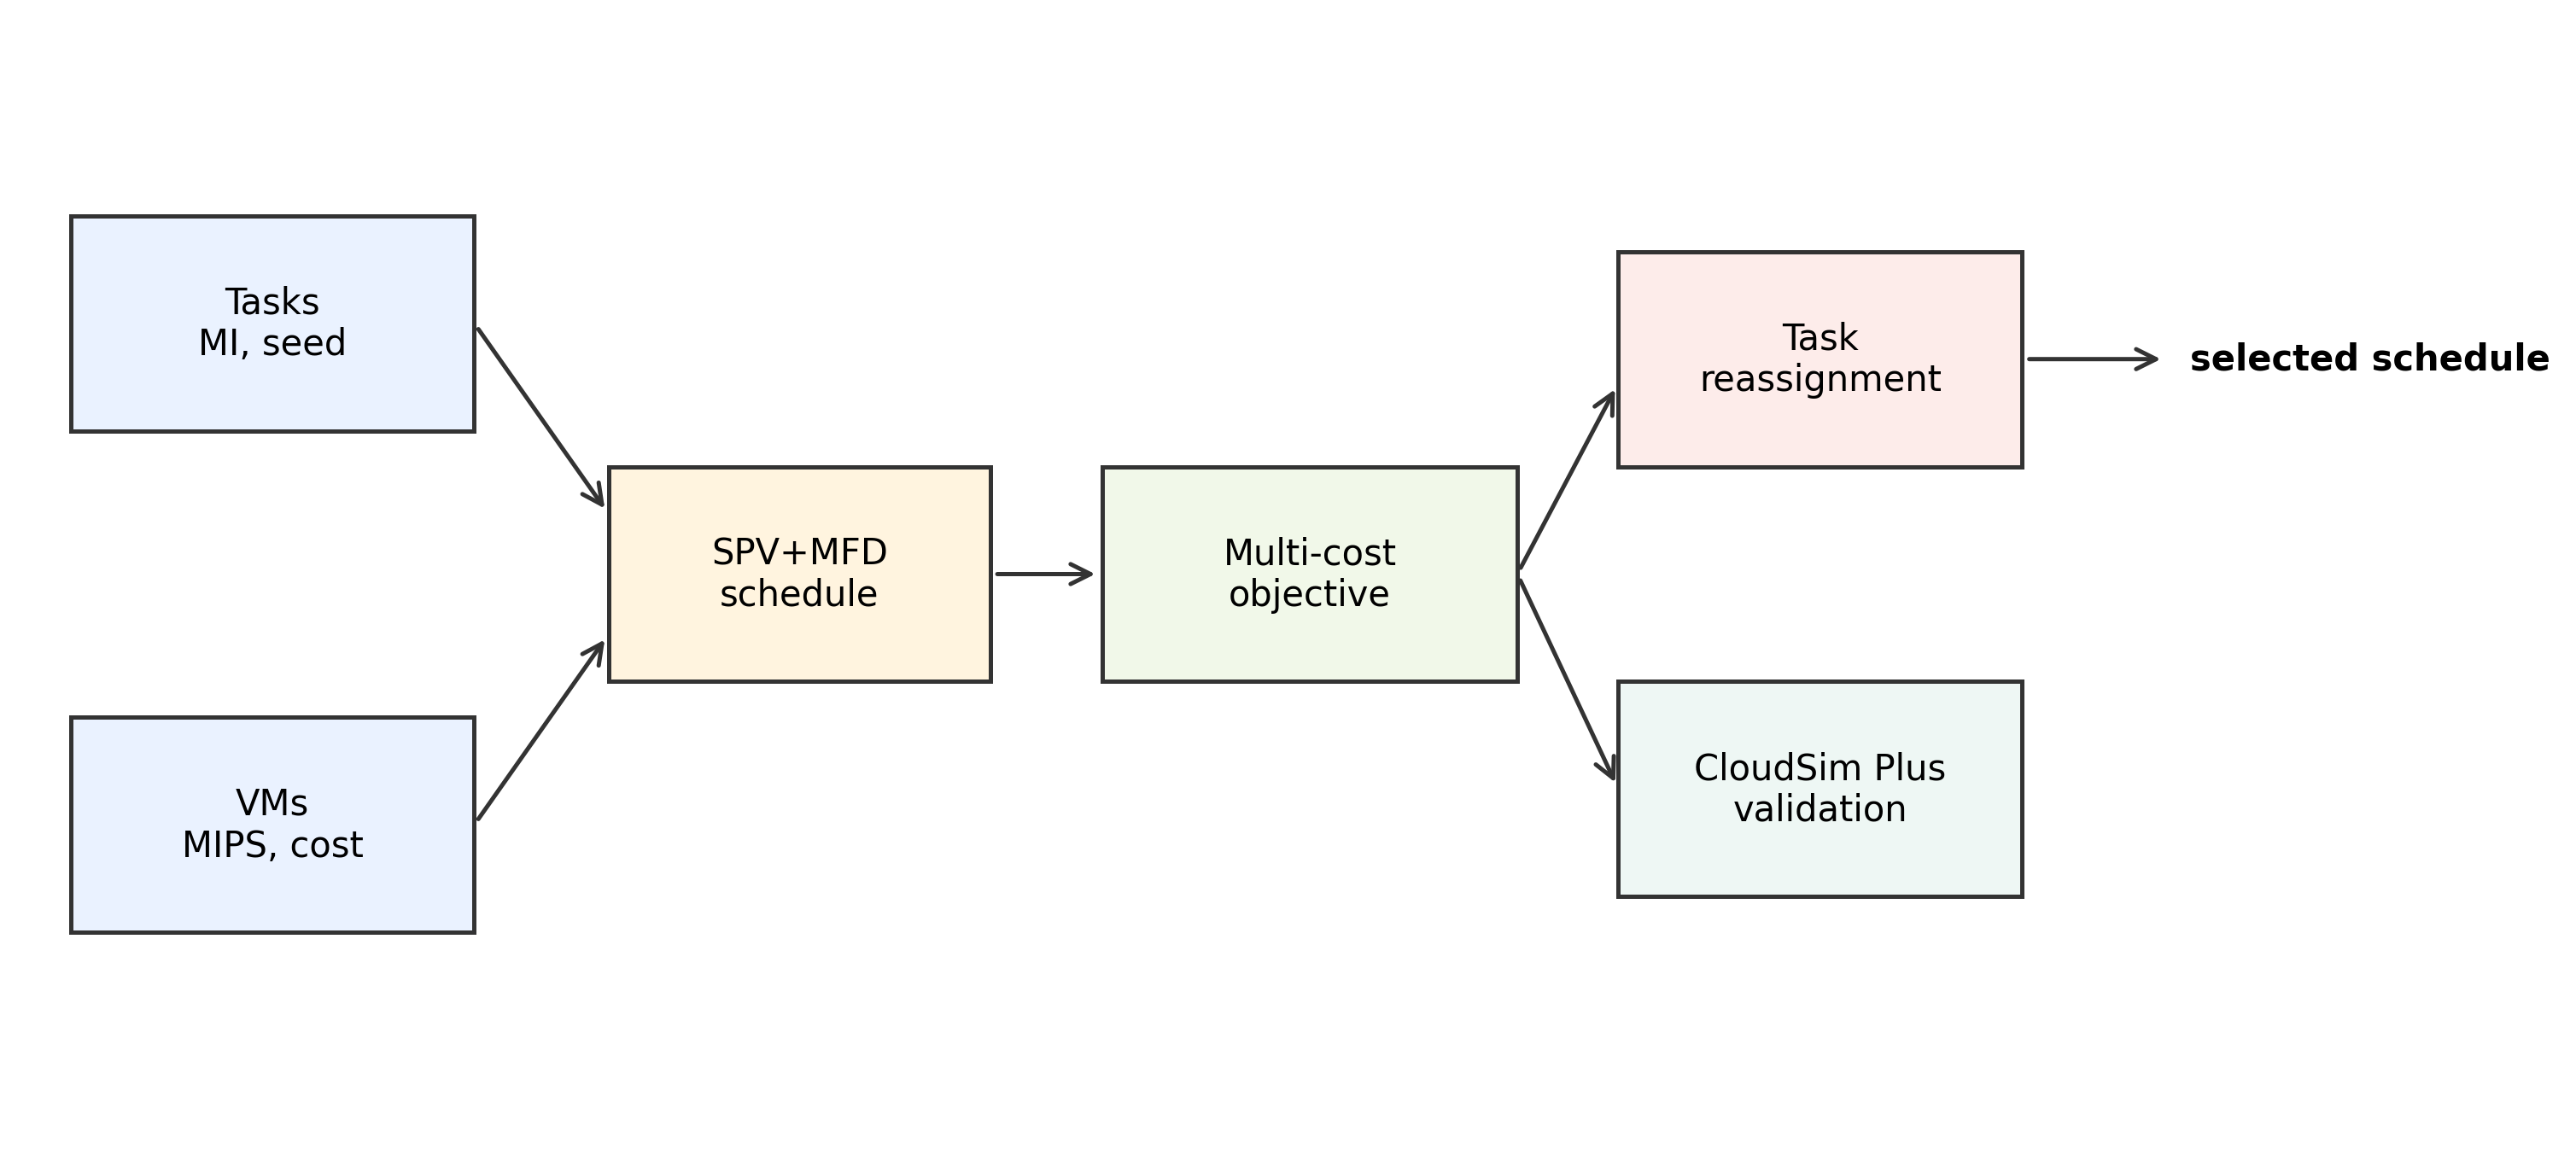
\includegraphics[width=0.92\textwidth]{figures/fig_lscbo_scheduling_model.png}
\caption{Multi-cost cloud task scheduling model used by LSCBO. A continuous population search is decoded into feasible task-to-VM assignments, evaluated by makespan, energy, execution cost, and load-balance criteria, and then improved by task-reassignment local search. The reported formal metrics use the stated analytical model, with CloudSim Plus used for implementation-level replay checks.}\label{fig:scheduling_model}
\end{figure}

\begin{table}[ht]
\centering
\caption{Main Notation for Cloud Task Scheduling}\label{tab:notation}
\begin{tabular}{l l}
\toprule
\textbf{Symbol} & \textbf{Description} \\
\midrule
$N$ & Number of cloud tasks \\
$M$ & Number of virtual machines \\
$MI_i$ & Million instructions of task $T_i$ \\
$MIPS_j$ & Processing speed of virtual machine $VM_j$ \\
$ETC_{i,j}$ & Expected execution time of task $T_i$ on $VM_j$ \\
$CT_j$ & Completion time of virtual machine $VM_j$ \\
$x_{i,j}$ & Binary task-assignment variable \\
$F$ & Scalarized scheduling objective \\
$w_k$ & Weight of the $k$-th scheduling criterion \\
$c_k$ & Greedy-LPT reference value used to normalize criterion $k$ \\
$B$, $B_g$, $B_{ls}$ & Total, global-search, and pair-reassignment evaluation budgets \\
\bottomrule
\end{tabular}
\end{table}

\subsection{Scheduling Criteria and Scalarized Objective}\label{sec4}
For schedule $x$, the completion time of VM $j$ is $CT_j=\sum_i ETC_{i,j}x_{i,j}$ and the makespan is $T_{ms}=\max_j CT_j$. Energy uses a nonlinear utilization model,
\begin{equation}
E=\sum_{j=1}^{M}\left[P^{idle}+(P^{max}-P^{idle})u_j^3\right]T_{ms}/3600,
\quad u_j=CT_j/T_{ms},
\end{equation}
where $P^{max}=250$ W and $P^{idle}=0.6P^{max}$. The cubic term avoids the exact linear dependence between energy and makespan in the earlier implementation.

Execution cost is $C=\sum_j r_jCT_j$. Rates span 0.05--0.20 cost units per unit time and follow
\begin{equation}
r_j=0.05+0.15\sqrt{\frac{MIPS_j-MIPS_{min}}{MIPS_{max}-MIPS_{min}}},
\end{equation}
so price is monotone in capacity but not exactly proportional to MIPS. Load balance is measured exactly as
\begin{equation}
\mathrm{LBR}=\frac{\sqrt{M^{-1}\sum_j(CT_j-\overline{CT})^2}}{\overline{CT}}.
\end{equation}

The scalar objective is
\begin{equation}
F=w_{ms}\frac{T_{ms}}{c_{ms}}+w_{en}\frac{E}{c_{en}}+w_{cost}\frac{C}{c_{cost}}+w_{lb}\frac{\mathrm{LBR}}{c_{lb}},
\end{equation}
where each $c_k$ is the corresponding value of the reported Greedy-LPT reference for the same workload and VM set. Normalizing all four criteria places the reference at one on every term, so the default equal weights give Greedy-LPT $F=1$. This also makes the weight profiles interpretable as relative priorities rather than coefficients applied to quantities with different numerical scales.

\subsection{Direct Assignment Representation and Common Warm Start}
A position $X\in[0,1]^N$ is decoded independently for each task:
\begin{equation}
x_i=\min\{M-1,\lfloor MX_i\rfloor\}.
\end{equation}
Every task-to-VM assignment has a corresponding vector, so the decoder does not force equal task counts across VMs. The deterministic reference sorts tasks by decreasing instruction length and assigns each task to the VM with the earliest projected finish time. Its schedule is encoded at interval midpoints, $X_i=(x_i+0.5)/M$, and inserted as the first individual for every population method. The remaining 29 individuals are random. This common warm start makes the comparison conservative: no population method can return a result worse than Greedy-LPT under elitist best tracking.

\section{The Proposed LSCBO Algorithm}\label{sec:algorithm}

\subsection{Continuous LSCBO Core}
The continuous core is identical in the CEC2017 and cloud implementations. A population of 30 is divided into coyote--badger pairs. During the first third of the core budget, the original tanh search is applied. During the second third, a two-coordinate rotation encircles the pair midpoint. During the final third, each individual moves halfway toward the best member of its half-population. In the first phase, an additional L\'{e}vy candidate is evaluated with probability $\rho_L=0.30$:
\begin{equation}
X_i^L=X_i+0.03\,\Delta\,\max(0.05,1-N_{eval}/B_g)L_i(1.5),
\end{equation}
where $L_i$ follows the Mantegna construction~\cite{Mantegna1994} and $\Delta$ is the coordinate span of the search domain. Thus $\Delta=200$ for the CEC2017 bounds $[-100,100]^D$ and $\Delta=1$ for the cloud decoder space $[0,1]^N$. The original CBO candidate and the additional L\'{e}vy candidate are separately counted and greedily accepted.

\subsection{Pareto-Safe Pair Reassignment}\label{sec:local_search}
The cloud run has a total budget $B=6000$. LSCBO allocates $B_g=600$ evaluations to its continuous core and the remaining $B_{ls}=5400$ to pair reassignment. The incumbent starts from the best schedule returned by the core. Local trials are processed in rounds of 400:
\begin{enumerate}
    \item sample two tasks assigned to different VMs and exchange their VM assignments;
    \item evaluate makespan, energy, cost, LBR, and $F$;
    \item declare the trial admissible only if all four component values are no greater than those of the incumbent;
    \item retain the admissible trial with the smallest $F$ in the round, then continue from it.
\end{enumerate}
The random stream used for pair sampling depends only on the workload, VM profile, seed, and weight profile. It is independent of the host optimizer and ablation label, which prevents different variants from receiving different local neighborhoods by accident.

Figure~\ref{fig:mechanism_workflow} summarizes the two budgeted stages. The continuous core retains the best schedule found under its 600-evaluation allowance, after which the pair search uses the remaining evaluations without accepting a trade-off in any of the four reported scheduling criteria.

\begin{figure*}[htbp]
\centering
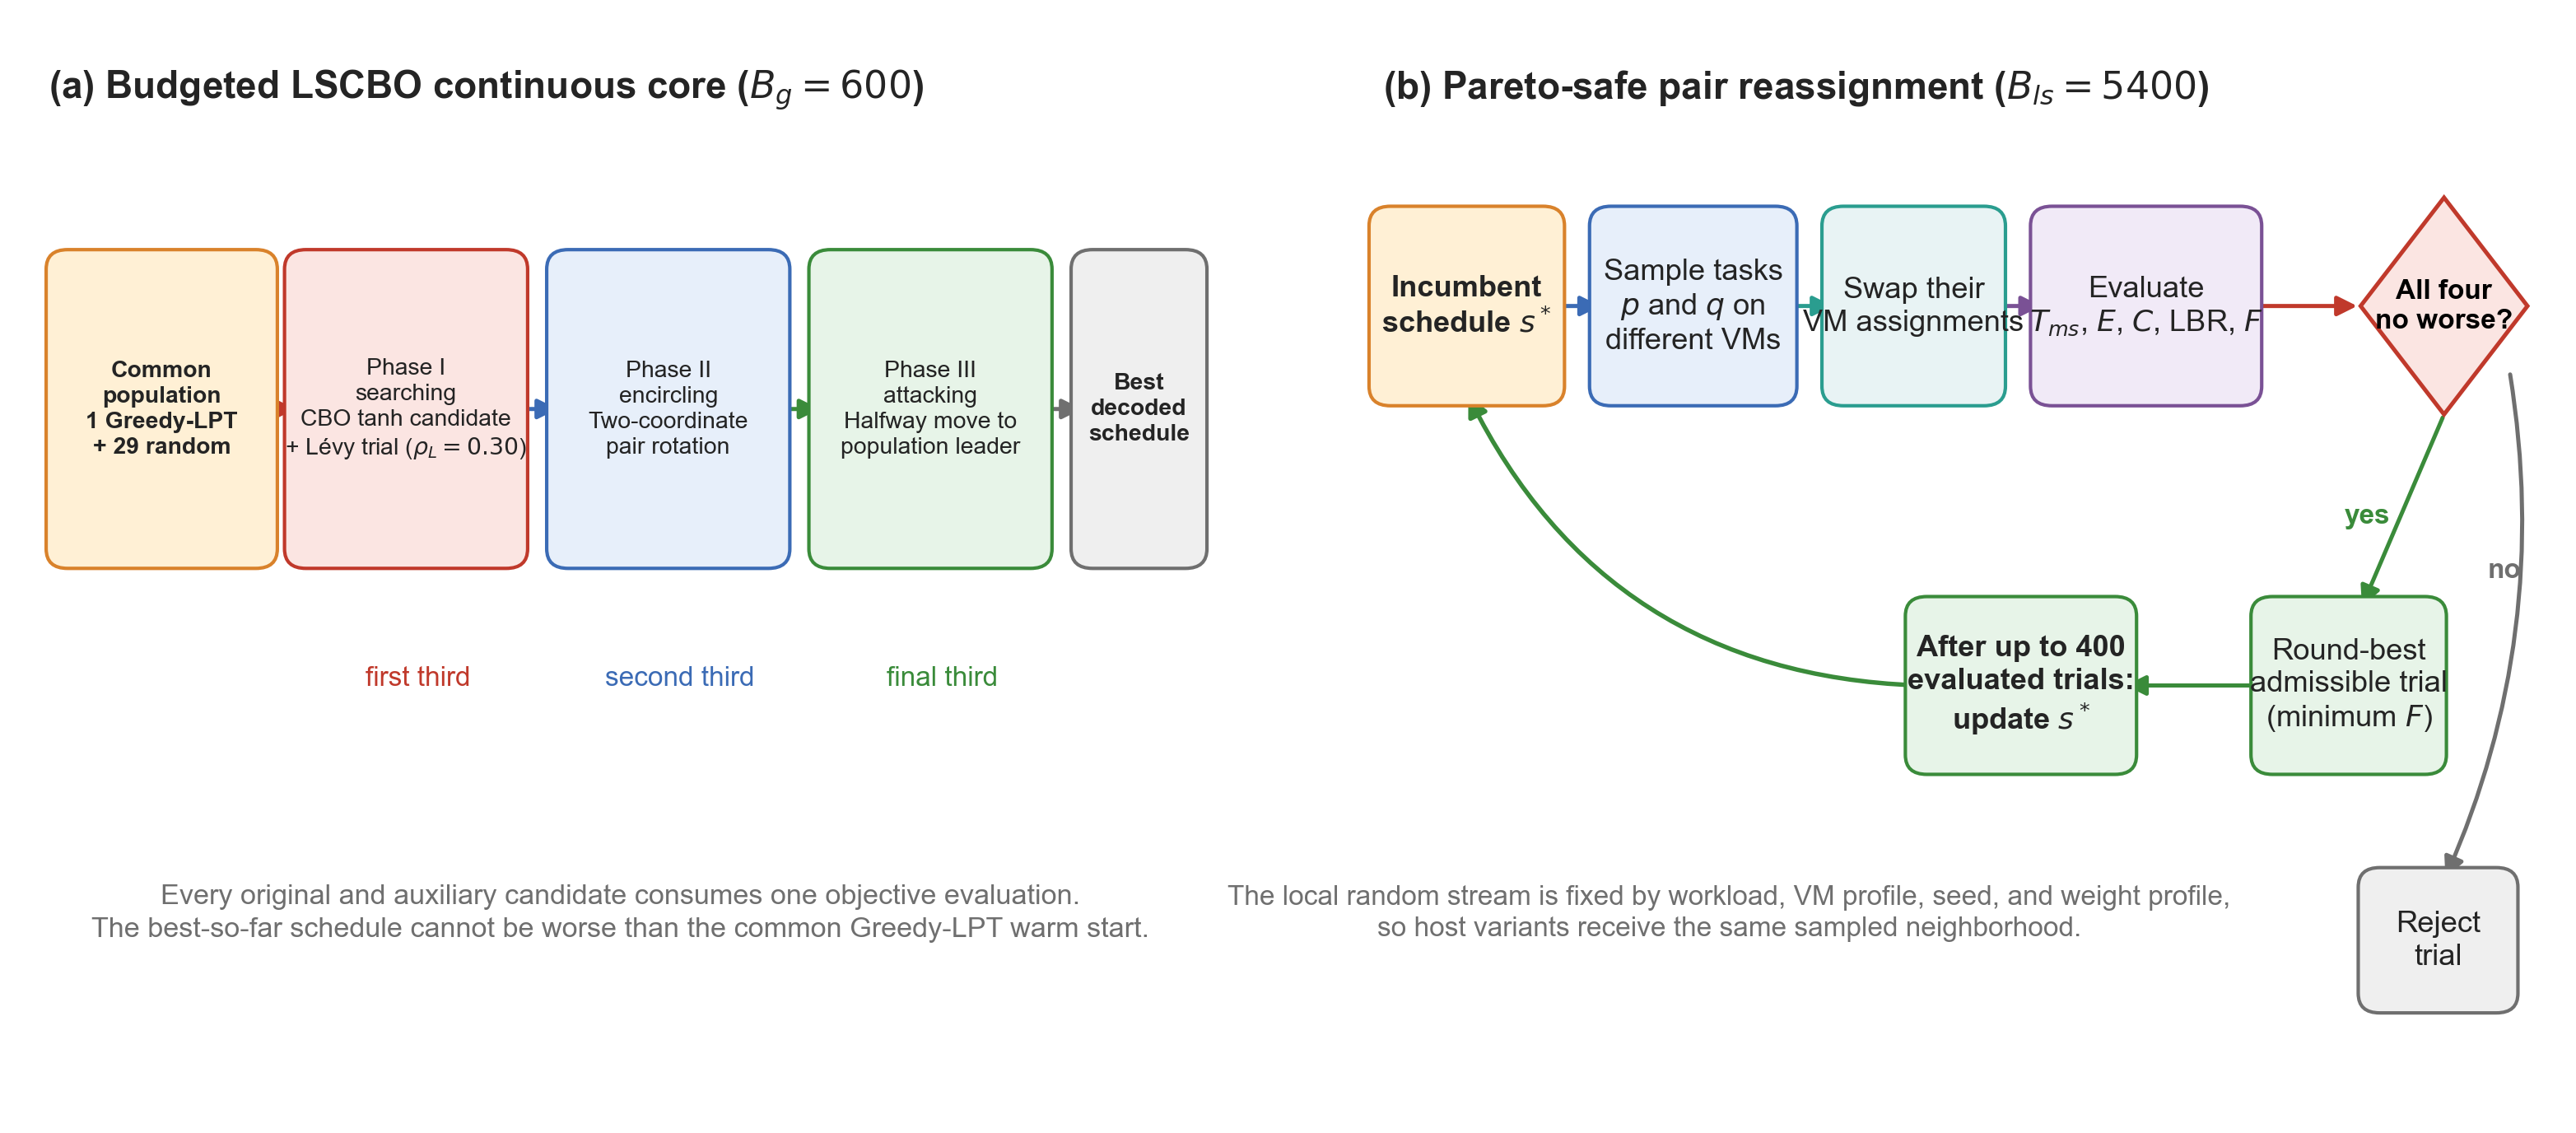
\includegraphics[width=0.98\textwidth]{figures/fig_lscbo_mechanism_workflow.png}
\caption{Budgeted LSCBO and Pareto-safe pair reassignment. (a) The continuous core progresses through searching, encircling, and attacking phases, with every original and auxiliary candidate counted against $B_g$. (b) A pair exchange is admissible only when makespan, energy, cost, and LBR are all non-worsening; the admissible trial with minimum $F$ updates the incumbent after each round.}\label{fig:mechanism_workflow}
\end{figure*}

\begin{algorithm}[ht]
\caption{Cloud LSCBO with Pareto-Safe Pair Reassignment}\label{alg:lscbo}
\begin{algorithmic}[1]
\State Build Greedy-LPT schedule $s_g$ and insert its encoding into all populations
\State Run the three-phase additive-L\'{e}vy LSCBO core for $B_g=600$ evaluations
\State $s^*\leftarrow$ best of the core and $s_g$
\While{total evaluations $<6000$}
    \State Sample and evaluate up to 400 task-pair exchanges from $s^*$
    \State Discard every trial that worsens any of makespan, energy, cost, or LBR
    \State $s^*\leftarrow$ admissible trial with minimum $F$, if one exists
\EndWhile
\State \textbf{Output:} $s^*$
\end{algorithmic}
\end{algorithm}

All population baselines receive 6,000 evaluations. LSCBO therefore does not receive extra objective calls for local search; its budget is partitioned between global and local components. Greedy-LPT is deterministic and requires one schedule evaluation.

\subsection{Computational Complexity}
Direct decoding costs $O(N)$ and a straightforward four-component evaluation costs $O(N+M)$. With a fixed evaluation budget $B$, a cloud run costs $O(B(N+M))$ and stores $O(SN)$ continuous coordinates for population size $S$. Pair reassignment is implemented by direct recomputation in the released program so that its counted evaluation is identical to an optimizer evaluation. The deterministic Greedy-LPT construction costs $O(N\log N+NM)$.

\section{Experimental Results}\label{sec5}

Two experimental series are kept separate. Series~1 evaluates the continuous LSCBO core on 29 official CEC2017 functions. Series~2 evaluates the cloud scheduler against five population methods and the deterministic Greedy-LPT reference. The reported cloud metrics are computed from the explicitly stated analytical model; CloudSim Plus is used as a replay-capable implementation layer and for smoke validation of schedule executability.

\begin{table}[ht]
\centering
\caption{Separation of the two validation series}\label{tab:series_boundary}
\begin{tabular}{p{0.18\textwidth} p{0.32\textwidth} p{0.40\textwidth}}
\toprule
\textbf{Series} & \textbf{Purpose and platform} & \textbf{Compared methods} \\
\midrule
Series~1 & Continuous global optimization on the official CEC2017 functions; no task-to-VM decoding or simulator is used. & LSCBO, CBO, PSO, GWO, WOA, SA, AOA, HLBO, and GWCA. \\
\midrule
Series~2 & Cloud task scheduling with direct assignment, a shared Greedy-LPT warm start, analytical multi-cost scoring, and CloudSim Plus replay support. & LSCBO, CBO, PSO, GWO, WOA, AOA, and Greedy-LPT under paired instances and explicit evaluation budgets. \\
\bottomrule
\end{tabular}
\end{table}

Task instances, VM instances, and random seeds are paired within each series. Table~\ref{tab:param_cec} summarizes the CEC2017 settings; cloud budgets and controls are stated in Section~\ref{sec:cloudsim_exp}.

\subsection{Experimental Series 1: CEC2017 Global Optimization Benchmarks}\label{sec:cec2017}

To validate LSCBO's fundamental optimization capability before applying it to the scheduling domain, we evaluate the algorithm on the CEC2017 benchmark suite, which comprises rotated and shifted test functions of varying complexity and modality. This two-tier evaluation strategy---benchmark validation followed by domain application---follows the established methodology in meta-heuristic research~\cite{Mirjalili2016,Khatab2025}. This series is intended as a general-capability validation rather than as a universal novelty claim in continuous optimization: its purpose is to confirm that the L\'{e}vy-modified search improves the base optimizer under the stated CEC2017 protocol before the algorithm is applied to its primary target domain, cloud task scheduling.

\subsubsection{CEC2017 Settings}
All CEC2017 experiments use the official C/C++ evaluator and its official $D=30$ shift, rotation, and shuffle data. The suite contains F1 and F3--F30 (29 functions; F2 is deprecated), with bounds $[-100,100]^D$~\cite{CEC2017}. Each algorithm--function cell is repeated for 30 paired seeds, and every run receives exactly 300,000 objective-function evaluations, including initialization and auxiliary trials. Population-based methods use 30 agents; SA is single-solution but receives the same evaluation budget. The comparison set is LSCBO, its CBO base, PSO~\cite{Kennedy1995}, GWO~\cite{Mirjalili2014}, WOA~\cite{Mirjalili2016}, SA~\cite{Kirkpatrick1983}, AOA~\cite{Abualigah2021}, HLBO~\cite{Dehghani2022HLBO}, and GWCA~\cite{Guan2023GWCA}.

\begin{table}[ht]
\centering
\caption{Parameter Settings for CEC2017 Experiments (Series~1)}\label{tab:param_cec}
\begin{tabular}{l l l}
\toprule
\textbf{Algorithm} & \textbf{Parameter} & \textbf{Value} \\
\midrule
LSCBO & Population size & 30 \\
       & L\'{e}vy stability $\beta$ & 1.5 \\
       & Trial fraction / step scale & 0.30 / 0.03 \\
\midrule
CBO & Population size & 30 \\
    & Rotation range $\theta_0$ & $\pi$ \\
    & Attack weight $w$ & 0.5 \\
\midrule
PSO & Population size & 30 \\
    & Inertia weight $w$ & $0.9 \rightarrow 0.4$ \\
    & Cognitive/social $c_1, c_2$ & 2.0, 2.0 \\
\midrule
SA & Initial temperature $T_0$ & 1,000 \\
   & Final temperature & $10^{-8}$ \\
\midrule
GWO & Population size & 30 \\
    & Convergence constant $a$ & $2 \rightarrow 0$ \\
\midrule
WOA & Population size & 30 \\
    & $a$, spiral $b$, branch probability & $2\!\rightarrow\!0$, 1, 0.5 \\
\midrule
AOA & Population size & 30 \\
    & $\alpha$, $\mu$, MOA & 5, 0.499, $0.2\!\rightarrow\!1$ \\
\midrule
HLBO & Population size & 30 \\
     & Local radius $R$ & 0.2 \\
\midrule
GWCA & Population size & 30 \\
     & $m,T,g,P,Q$ & 3, 8.3, 9.8, 9, 6 \\
\midrule
\multicolumn{3}{l}{\footnotesize{All methods: $D=30$, bounds $[-100,100]^D$, 30 paired runs, 300,000 evaluations per run.}} \\
\bottomrule
\end{tabular}
\end{table}

\subsubsection{Contribution of the Additive L\'{e}vy Trial}\label{sec:cec_levy_ablation}
Pair reassignment is not used on continuous benchmarks. In the official CEC2017 implementation, LSCBO and CBO share the same population size, three CBO phases, greedy replacement, and evaluation budget; the additional L\'{e}vy trial is their only algorithmic difference. LSCBO has a lower per-function mean error than CBO on all 29 functions. The paired cross-function Wilcoxon test remains significant after Holm correction ($p=2.16\times10^{-5}$). This matched comparison supports the limited conclusion that the additive L\'{e}vy trial improves the CBO core under the stated CEC2017 protocol. It does not establish universal superiority of the resulting optimizer.

Table~\ref{tab:cec_external} reports the complete official comparison. LSCBO obtains the best average rank (1.690) over the 29 functions, ahead of SA (2.655) and PSO (3.345). The omnibus statistics are $\chi^2=160.313$ for the Friedman test and $F=62.616$ for the Iman--Davenport correction ($p=6.18\times10^{-53}$)~\cite{Friedman1937,ImanDavenport1980}. Pairwise Wilcoxon tests are performed on the 29 per-function mean errors, not on 870 pooled runs~\cite{Wilcoxon1945}. After Holm correction, LSCBO differs from CBO, PSO, GWO, WOA, AOA, HLBO, and GWCA ($p\leq0.0011$), but not from SA ($p=0.066$). The Nemenyi critical difference is approximately 2.23; the rank gaps to SA (0.97) and PSO (1.66) remain below it. We therefore report LSCBO as first by average rank, not as significantly superior to every comparator.

\begin{table}[ht]
\centering
\caption{Official CEC2017 comparison: Friedman average rank (29 functions, 30 runs, 300,000 evaluations per run; lower is better)}\label{tab:cec_external}
\begin{tabular}{l c}
\toprule
\textbf{Algorithm} & \textbf{Average rank} \\
\midrule
\textbf{LSCBO} & \textbf{1.690} \\
SA             & 2.655 \\
PSO            & 3.345 \\
HLBO           & 4.621 \\
GWCA           & 4.793 \\
CBO            & 5.034 \\
GWO            & 6.862 \\
AOA            & 7.448 \\
WOA            & 8.552 \\
\bottomrule
\end{tabular}
\end{table}

\begin{figure}[htbp]
\centering
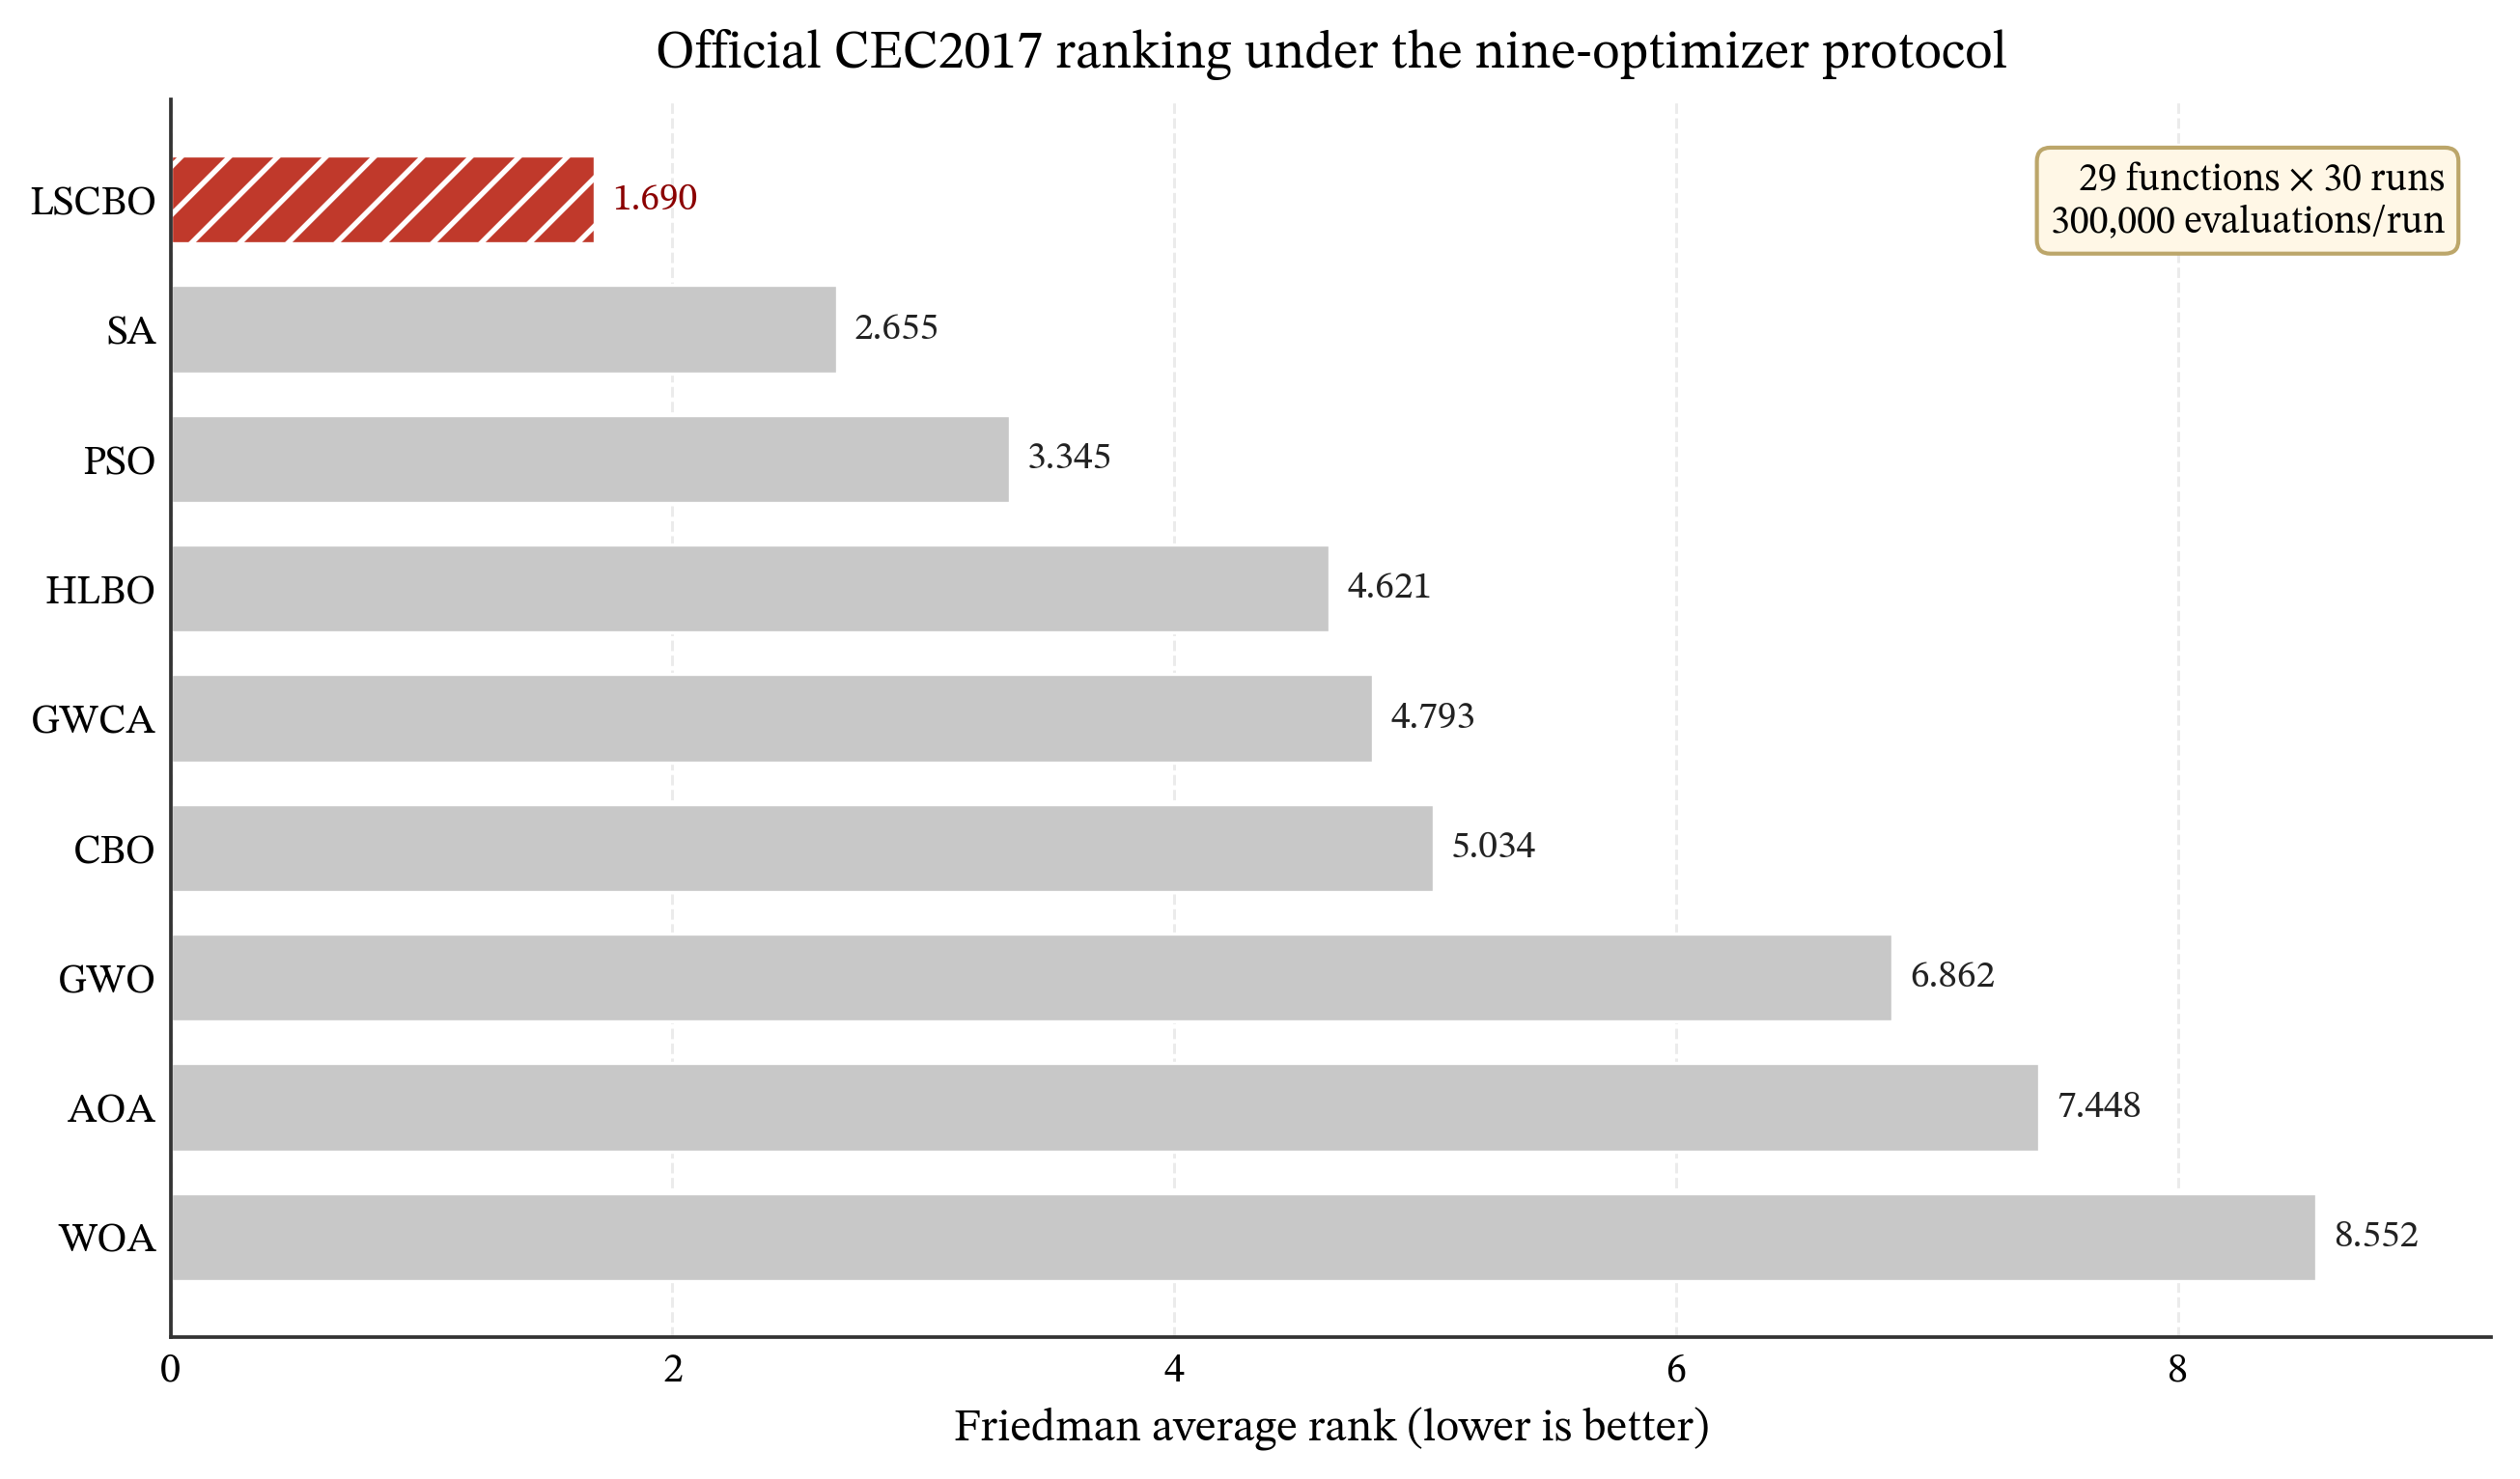
\includegraphics[width=0.90\textwidth]{figures/fig1_cec_ranking.png}
\caption{Official CEC2017 average-rank comparison under the nine-optimizer protocol. LSCBO obtains the best Friedman average rank (1.690) over the 29-function, 30-run, 300,000-evaluation setting; lower rank indicates better performance.}\label{fig:cec_ranking}
\end{figure}

\noindent No function is omitted. The ranking is computed from the complete 7,830-run result set; per-run values, per-function summaries, convergence checkpoints, and paired statistical outputs are included in the reproducibility package.

\subsubsection{Convergence Analysis on CEC2017}
Figure~\ref{fig:cec_convergence} reports all saved checkpoints under the complete 29-function protocol rather than selecting individual functions. LSCBO's mean cross-function rank improves as the evaluation budget is consumed and reaches the final rank of 1.690 reported in Table~\ref{tab:cec_external}. Figure~\ref{fig:cec_function_convergence} complements the aggregate rank curve with representative function-level traces. These trajectories are descriptive; the final paired tests remain the basis for statistical comparison.

\begin{figure*}[htbp]
\centering
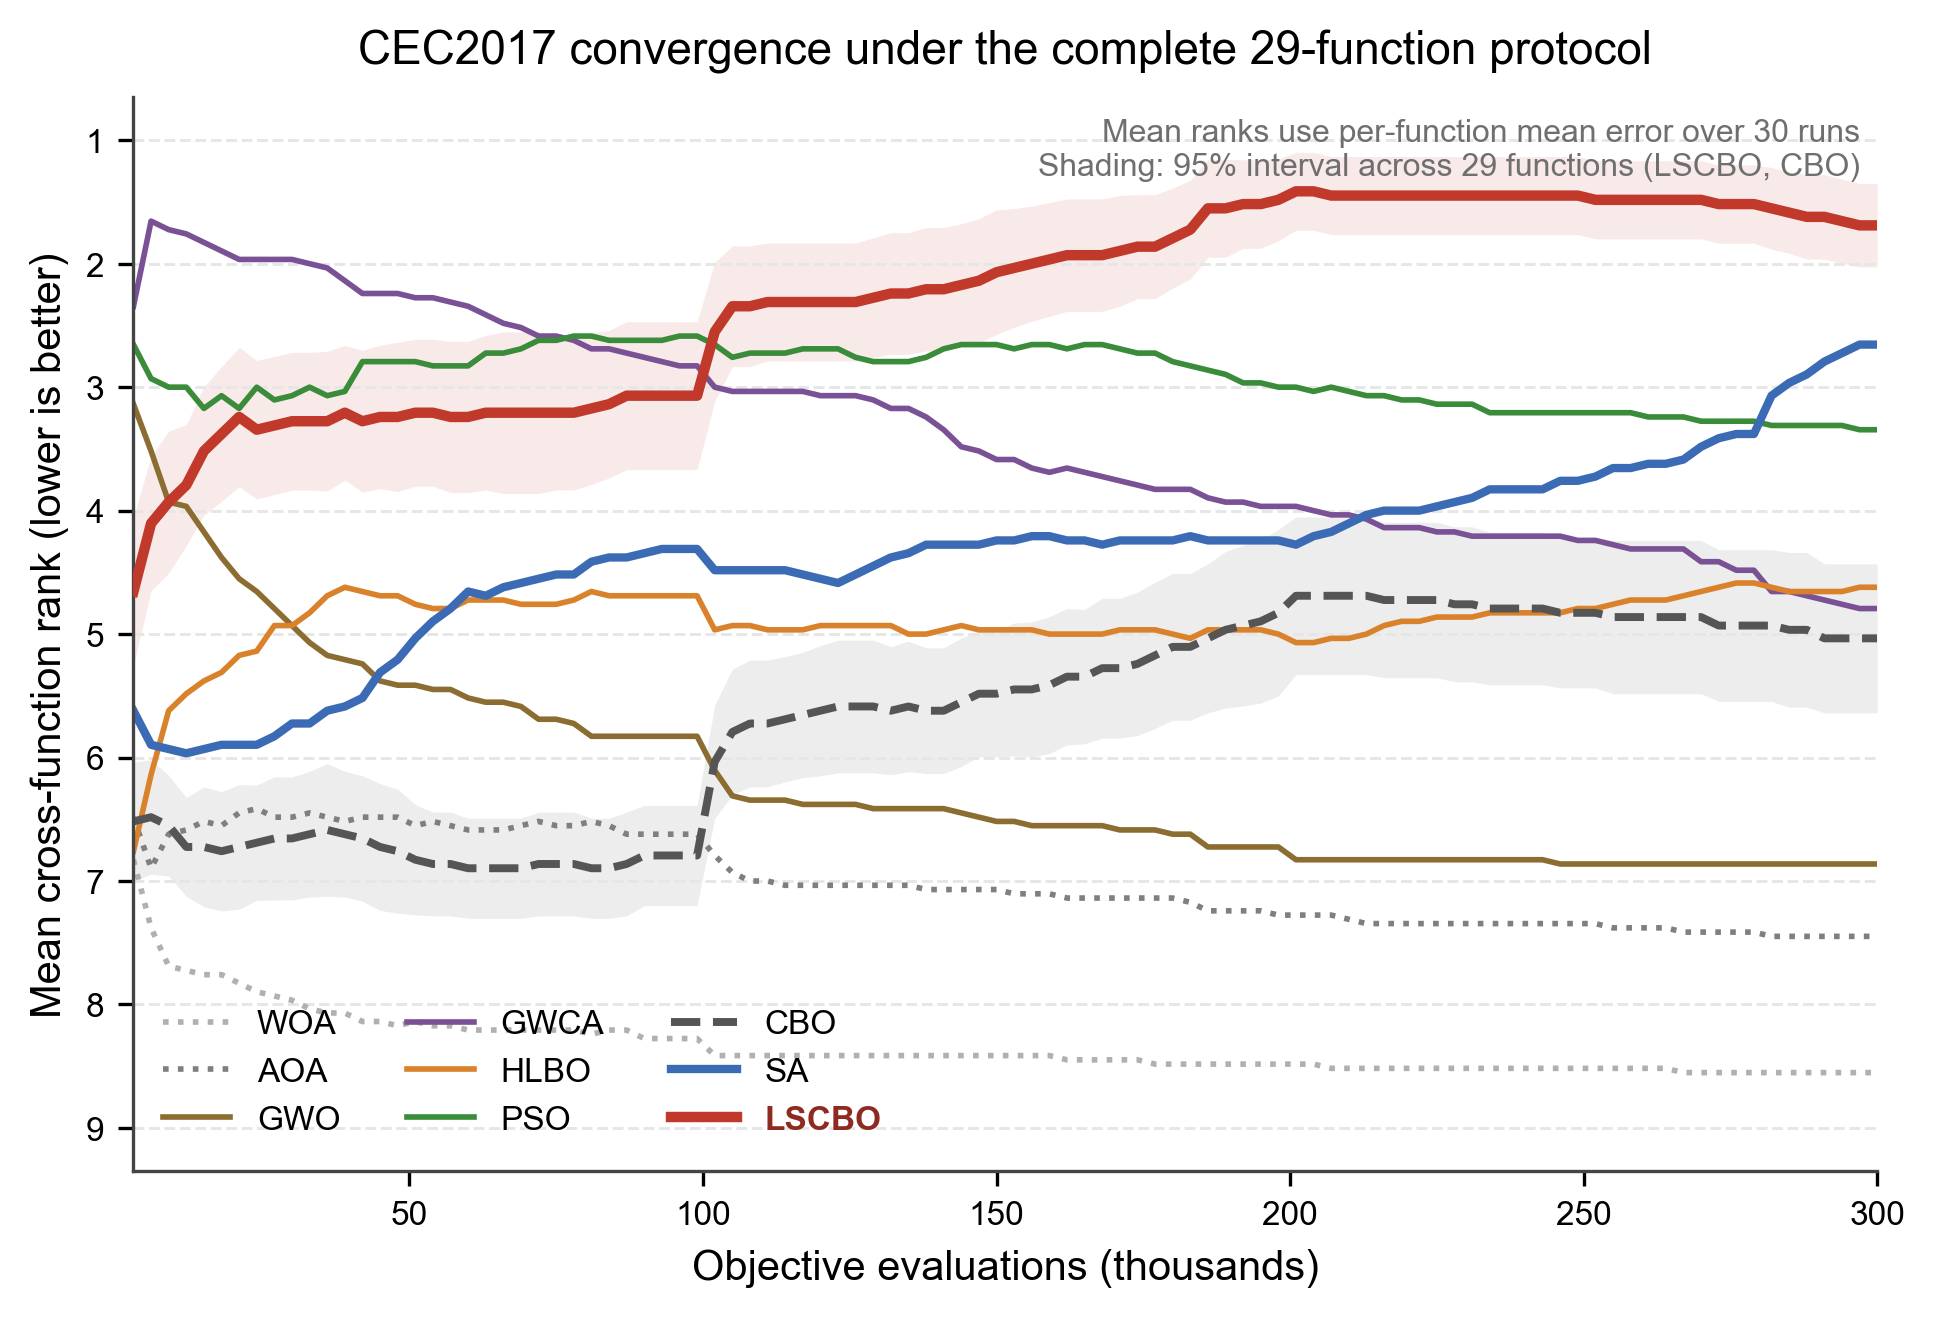
\includegraphics[width=0.78\textwidth]{figures/fig_cec_convergence_rank.png}
\caption{CEC2017 convergence over all 29 functions. At each checkpoint, the 30-run mean error is ranked among the nine methods within each function, and the curves average those 29 ranks. Lower is better. Shading gives 95\% intervals across functions for LSCBO and CBO.}\label{fig:cec_convergence}
\end{figure*}

\begin{figure*}[htbp]
\centering
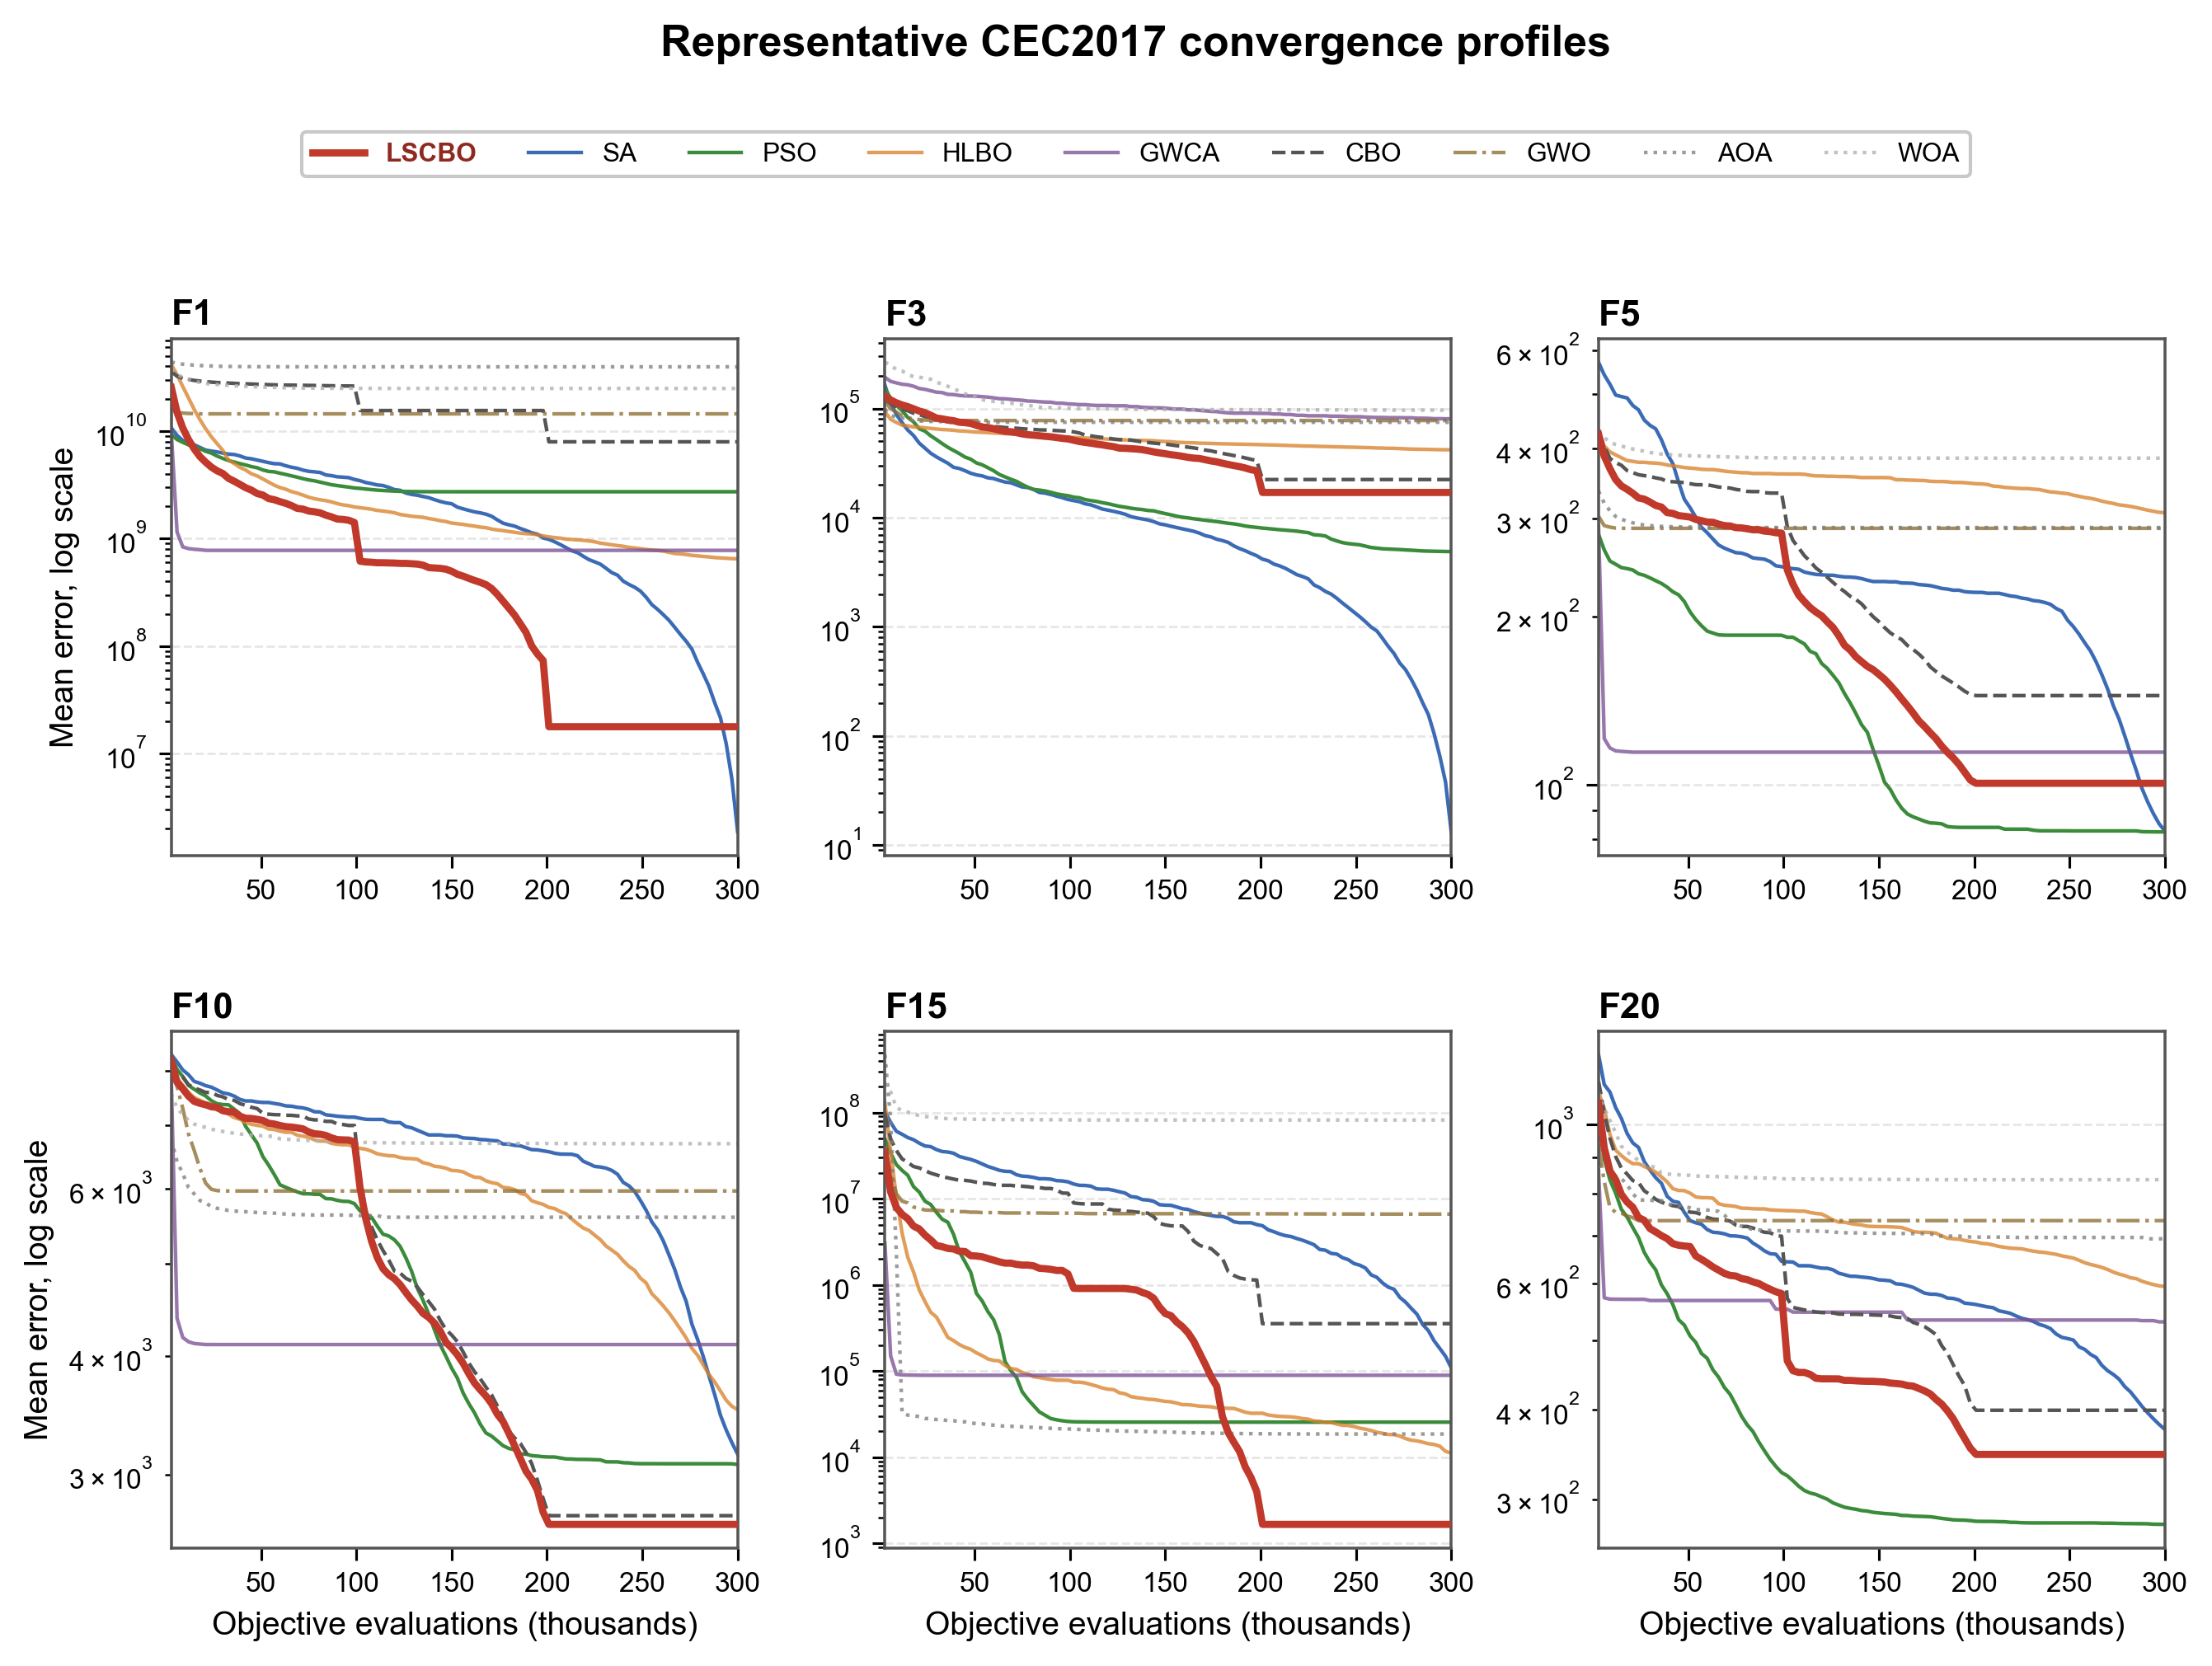
\includegraphics[width=\textwidth]{figures/fig_cec_function_convergence_grid.png}
\caption{Representative CEC2017 convergence profiles. Six functions are shown to make the checkpoint dynamics visible without replacing the complete-protocol ranking in Figure~\ref{fig:cec_convergence}. Each curve is the 30-run mean error for one optimizer; the vertical axis uses a log scale.}\label{fig:cec_function_convergence}
\end{figure*}

\subsection{Experimental Series 2: Cloud Task Scheduling}\label{sec:cloudsim_exp}

\subsubsection{Protocol and Simulator}
The cloud implementation includes a CloudSim Plus 8.0.0 replay path~\cite{Calheiros2011,SilvaFilho2017}. Each scenario contains 50 VMs, task lengths sampled uniformly from 1,000 to 20,000 MI, and seeds 43--72. The default VM range is 500--2,000 MIPS. The datacenter expands beyond 10 four-core hosts when required; hosts provide 16 GB RAM, 1 TB storage, and 10 Gbps bandwidth. Hosts and VMs use TimeShared policies. The formal tables below report the analytical multi-cost objective defined in Section~\ref{sec3}; the replay path is retained to check that generated assignments are executable in the simulator.

The main comparison uses $N\in\{200,500,1000,2000,5000\}$ and 30 paired seeds. LSCBO, CBO, PSO, GWO, WOA, and AOA use population 30 and exactly 6,000 objective evaluations. Greedy-LPT is deterministic and uses one evaluation. All population methods receive the same Greedy-LPT schedule as their first individual and use the direct decoder in Section~\ref{sec:algorithm}. PSO uses $w:0.9\rightarrow0.4$ and $c_1=c_2=2$; GWO uses $a:2\rightarrow0$; WOA uses its standard encircling and logarithmic-spiral branches; AOA uses $\alpha=5$, $\mu=0.499$, and MOA $0.2\rightarrow1$. These settings are shared with the tested CEC implementations.

The canonical analytic dataset contains 5,310 rows: 1,050 main-comparison rows, 1,200 ablation rows, 2,250 weight-sensitivity rows, and 810 VM-heterogeneity rows. The released verifier checks row counts, paired blocks, duplicate keys, finite values, evaluation budgets, and the no-regression invariant. A small CloudSim Plus smoke replay is used as an implementation sanity check; full replay of every formal row is left as a reproducibility extension rather than used as evidence for the numerical claims in this version.

\subsubsection{Main Comparison}
Table~\ref{tab:cloud_main_objective} reports mean objective values after all four criteria are normalized by the Greedy-LPT reference. GWO, WOA, and AOA return the warm start in every block. CBO and PSO each find a lower objective in one of 150 blocks, but their aggregate changes are below 0.002\%. LSCBO with pair reassignment improves all 150 blocks. This result should not be read as evidence that its population search is stronger: the matched ablation below attributes the repeatable difference to pair reassignment.

\begin{table*}[ht]
\centering
\caption{Mean scalar objective over 30 paired seeds (lower is better)}\label{tab:cloud_main_objective}
\resizebox{\textwidth}{!}{%
\begin{tabular}{l c c c c c}
\toprule
\textbf{Method} & $N=200$ & $N=500$ & $N=1000$ & $N=2000$ & $N=5000$ \\
\midrule
\textbf{LSCBO + Pareto-safe pair search} & \textbf{0.982632} & \textbf{0.982617} & \textbf{0.983700} & \textbf{0.983444} & \textbf{0.985240} \\
CBO & 1.000000 & 0.999937 & 1.000000 & 1.000000 & 1.000000 \\
PSO & 0.999929 & 1.000000 & 1.000000 & 1.000000 & 1.000000 \\
GWO / WOA / AOA / Greedy-LPT & 1.000000 & 1.000000 & 1.000000 & 1.000000 & 1.000000 \\
\bottomrule
\end{tabular}
}
\end{table*}

\begin{table*}[ht]
\centering
\caption{Relative improvement of LSCBO over Greedy-LPT computed from scale-wise mean component values. Parentheses give paired wins out of 30 seeds; all remaining cases are ties, with no component losses.}\label{tab:main_improvement}
\resizebox{\textwidth}{!}{%
\begin{tabular}{l c c c c c}
\toprule
\textbf{Scale} & \textbf{Makespan} & \textbf{Energy} & \textbf{Cost} & \textbf{LBR} & \textbf{Objective} \\
\midrule
$N=200$  & 0.0124\% (8)  & 0.0694\% (30) & 0.0250\% (30) & 6.8139\% (30) & 1.7368\% (30) \\
$N=500$  & 0.0009\% (5)  & 0.0186\% (30) & 0.0058\% (30) & 6.6074\% (30) & 1.7383\% (30) \\
$N=1000$ & 0.0005\% (4)  & 0.0083\% (30) & 0.0028\% (30) & 6.2843\% (30) & 1.6300\% (30) \\
$N=2000$ & 0.0004\% (7)  & 0.0039\% (30) & 0.0013\% (30) & 6.4391\% (30) & 1.6556\% (30) \\
$N=5000$ & 0.0002\% (10) & 0.0014\% (30) & 0.0005\% (30) & 5.6472\% (30) & 1.4760\% (30) \\
\bottomrule
\end{tabular}
}
\end{table*}

The no-regression rule is visible in Table~\ref{tab:main_improvement}: all mean changes are nonnegative and there are no component losses in any block. The practical effect is concentrated in LBR. Objective reductions are consistent but small and decline with task count. Figures~\ref{fig:cloud_small_scale_costs} and~\ref{fig:cloud_large_scale_costs} follow the task-scale cost-profile style used in recent cloud-scheduling studies: all method groups move with the workload scale, while the small vertical separations show that the reported improvement is a refinement on top of a strong Greedy-LPT warm start. GWO, WOA, and AOA coincide with Greedy-LPT under this protocol, so they are grouped rather than redrawn as identical traces.

\begin{figure*}[htbp]
\centering
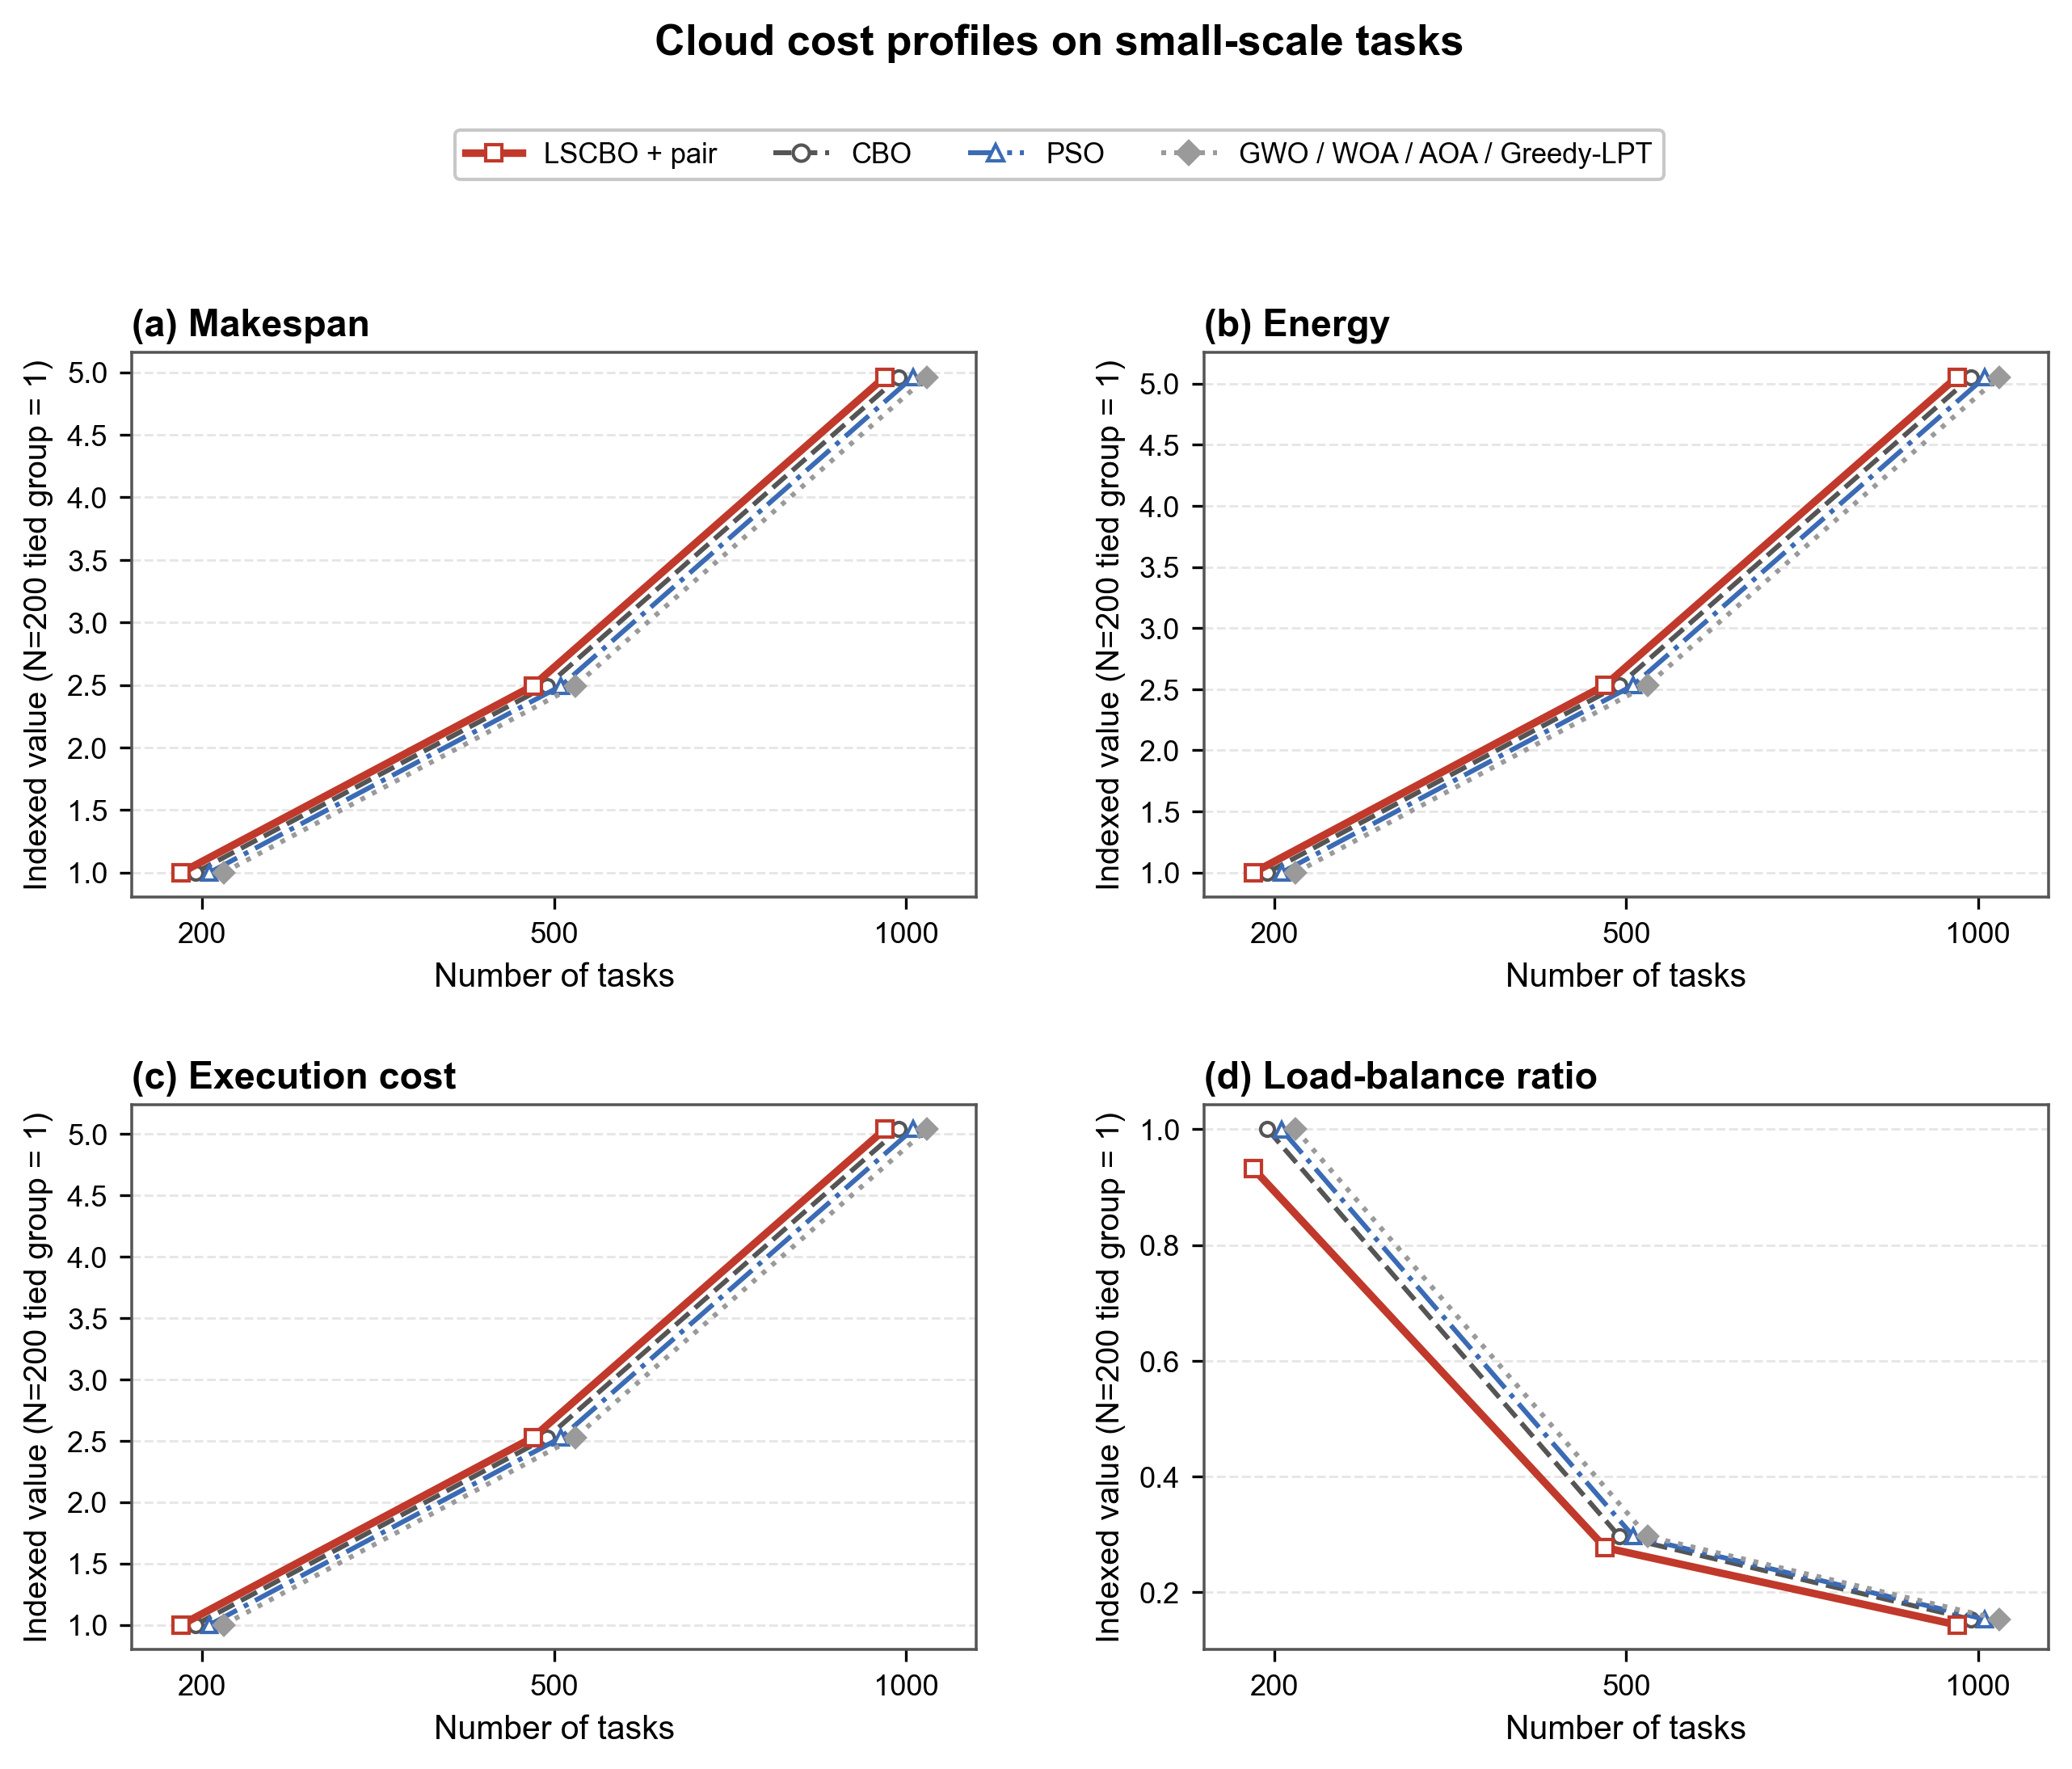
\includegraphics[width=0.95\textwidth]{figures/fig_cloud_small_scale_cost_profiles.png}
\caption{Small-scale cloud cost profiles. Values are indexed to the GWO/WOA/AOA/Greedy-LPT tied group at $N=200$ within each component. Horizontal positions are slightly dodged only to reveal overlapping traces; vertical values are unchanged.}\label{fig:cloud_small_scale_costs}
\end{figure*}

\begin{figure*}[htbp]
\centering
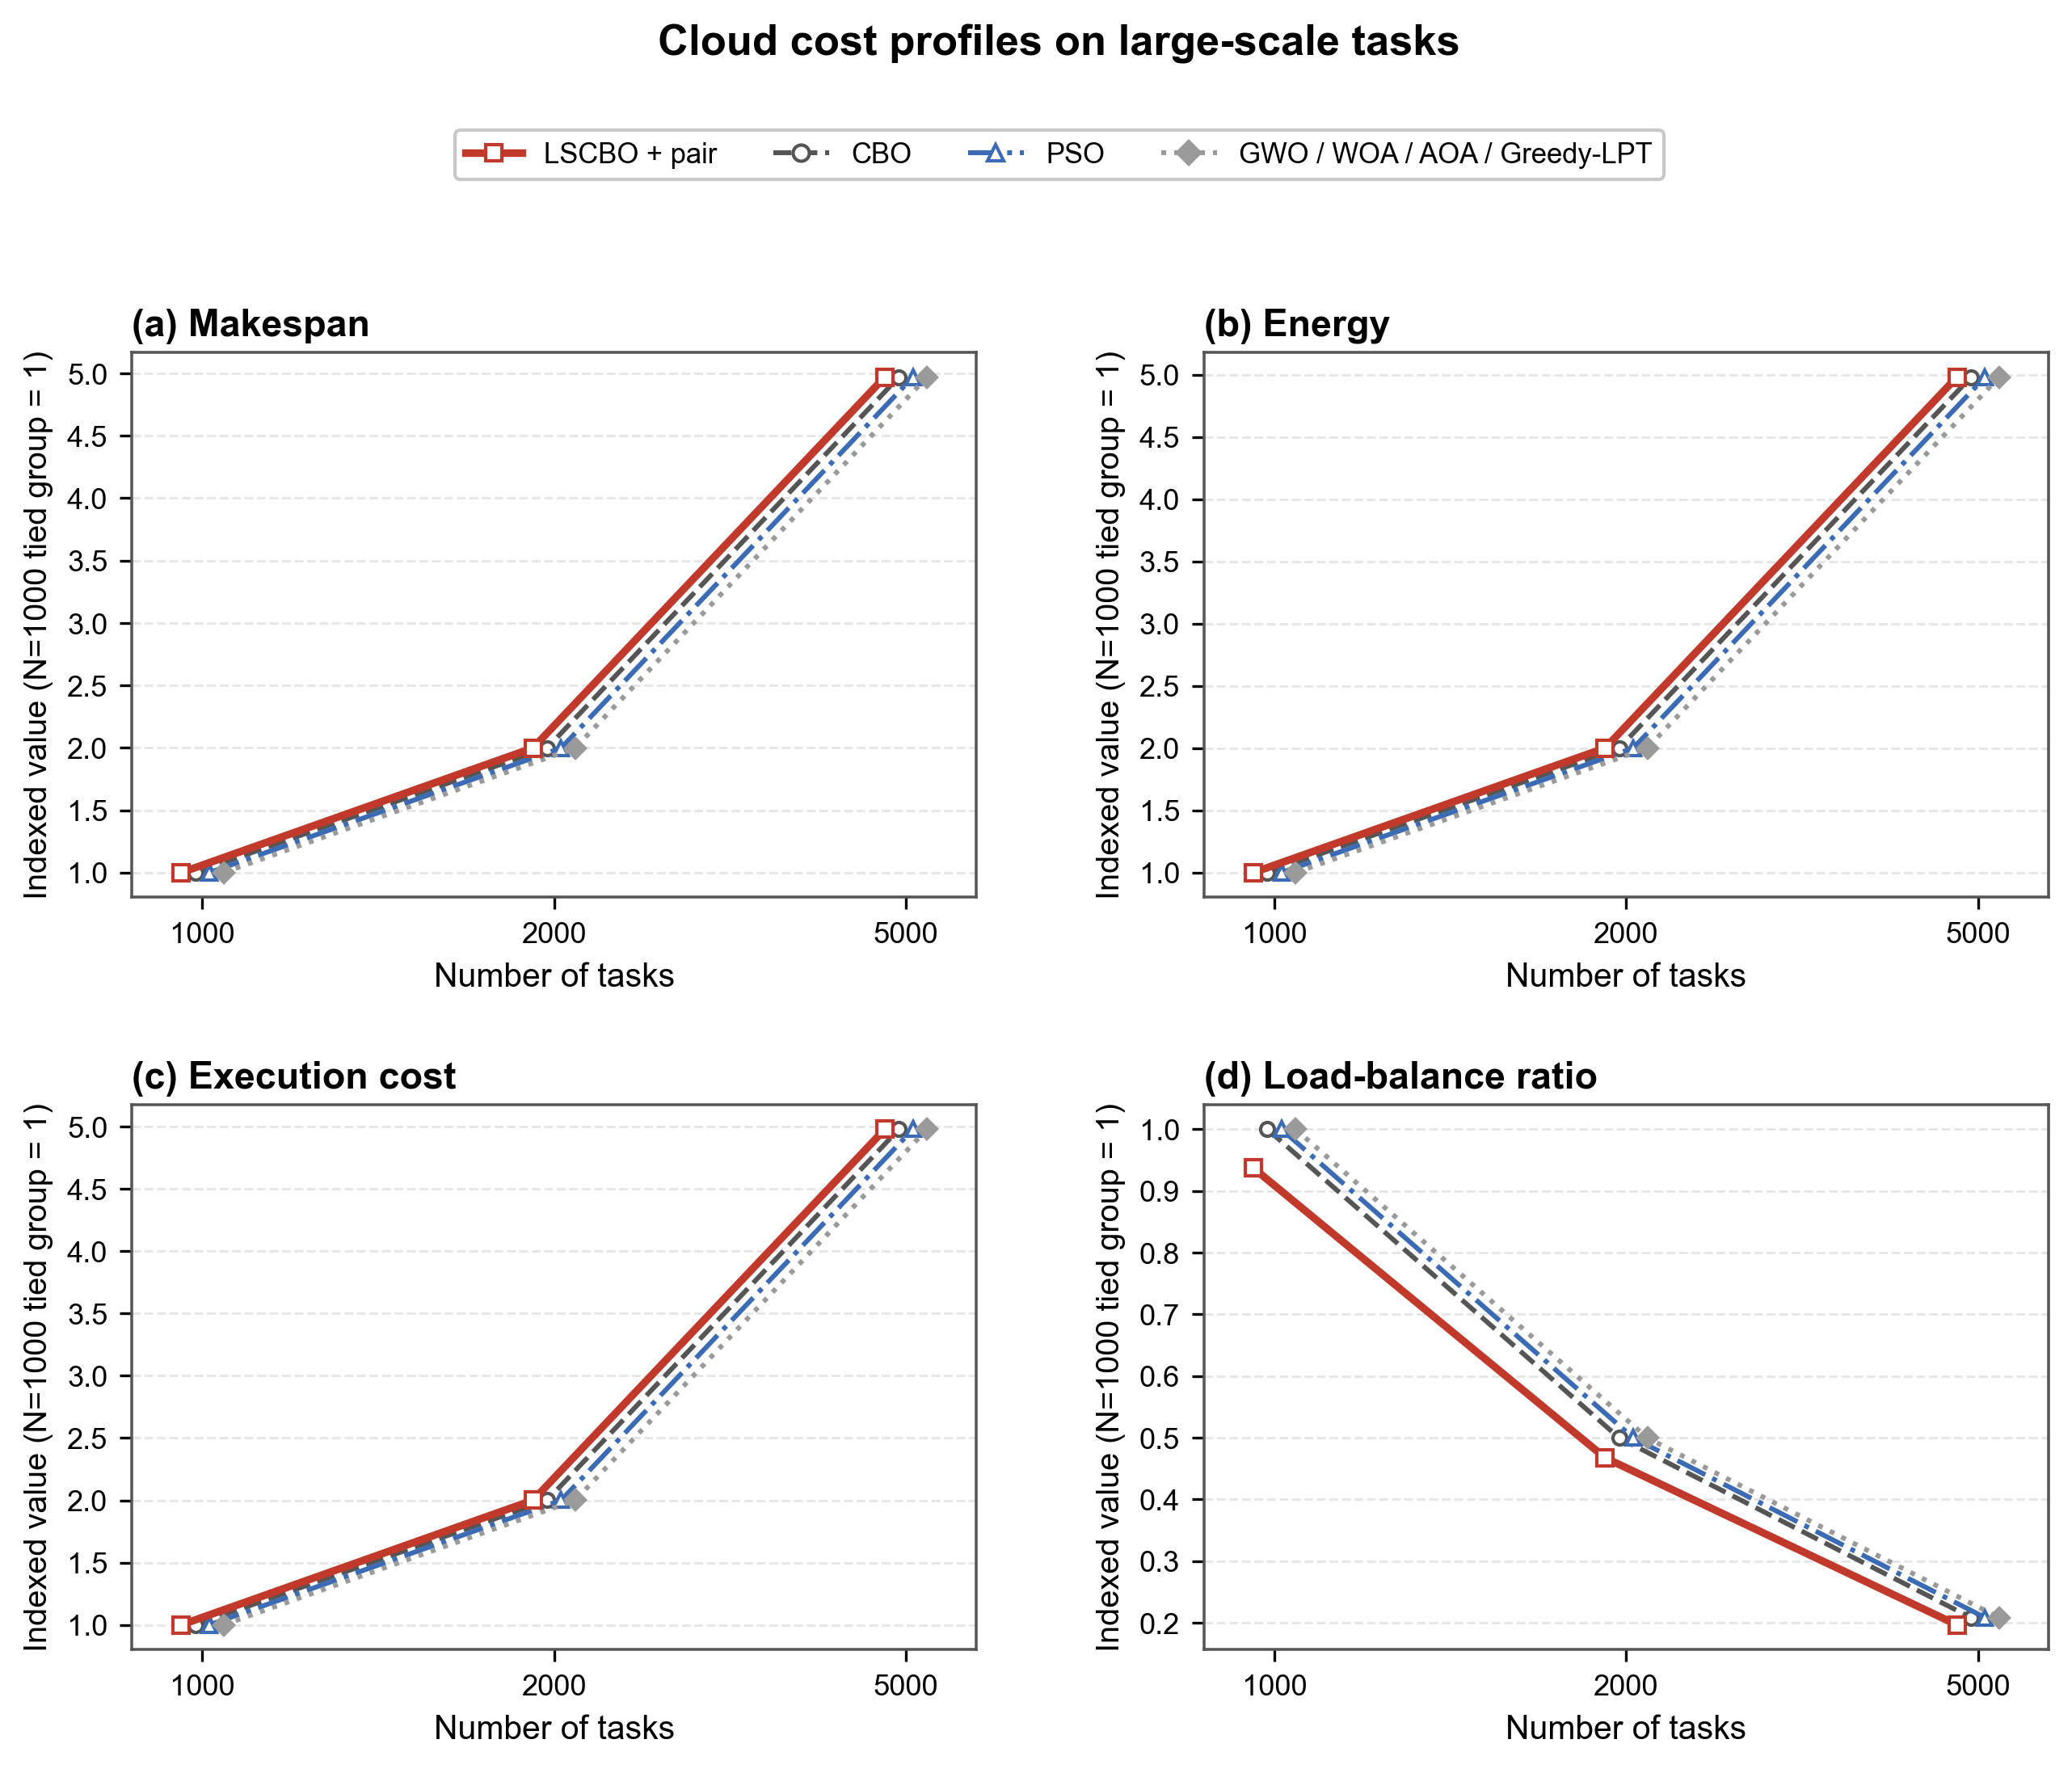
\includegraphics[width=0.95\textwidth]{figures/fig_cloud_large_scale_cost_profiles.png}
\caption{Large-scale cloud cost profiles. Values are indexed to the GWO/WOA/AOA/Greedy-LPT tied group at $N=1000$ within each component. The plots show workload scaling and component behavior, while Table~\ref{tab:main_improvement} reports the paired improvement magnitudes.}\label{fig:cloud_large_scale_costs}
\end{figure*}

\FloatBarrier

For the scalar objective, the Friedman test across the seven methods gives $\chi^2=887.615$ and $p=1.79\times10^{-188}$. Two-sided Wilcoxon tests give 149 wins and one loss against CBO, and 150 wins against each other comparator; every Holm-adjusted value is at most $1.38\times10^{-25}$. These small $p$-values indicate consistency rather than a large physical reduction in makespan, energy, or cost. Against Greedy-LPT, the median paired objective difference is $-0.0146$ on a reference-normalized scale where the baseline is one.

\subsubsection{Mechanism Ablation}\label{sec:phase_ablation}
Table~\ref{tab:phase_ablation} averages 150 paired blocks per variant. LSCBO, no-L\'{e}vy CBO, and local search alone are numerically identical because their global phases do not improve the common Greedy-LPT start. Removing local search returns the reference schedule. A single-task Pareto-safe relocation also makes no improvement, showing that the pair neighborhood, rather than simple movement from a loaded to an underloaded VM, is necessary. Objective-only pair search obtains a lower scalar value but slightly worsens mean energy and cost; Pareto-safe acceptance deliberately rejects such trade-offs.

\begin{table*}[ht]
\centering
\caption{Canonical cloud ablation (mean over 150 paired blocks)}\label{tab:phase_ablation}
\resizebox{\textwidth}{!}{%
\begin{tabular}{l c c c c c}
\toprule
\textbf{Variant} & \textbf{Makespan} & \textbf{Energy} & \textbf{Cost} & \textbf{LBR} & \textbf{Objective} \\
\midrule
Objective-only pair search & 291.5198 & 1010.6213 & 2193.7017 & 0.002337 & 0.899351 \\
\textbf{Pareto-safe pair search (LSCBO)} & \textbf{291.5373} & \textbf{1010.3976} & \textbf{2193.5747} & \textbf{0.003671} & \textbf{0.983527} \\
No L\'{e}vy / pair search only & 291.5373 & 1010.3976 & 2193.5747 & 0.003671 & 0.983527 \\
No local search / CBO / Greedy-LPT & 291.5391 & 1010.4510 & 2193.6144 & 0.003934 & 1.000000 \\
Pareto-safe single relocation & 291.5391 & 1010.4510 & 2193.6144 & 0.003934 & 1.000000 \\
\bottomrule
\end{tabular}
}
\end{table*}

\subsubsection{Weight Sensitivity}\label{sec:weight_sensitivity}
Five profiles are tested over $N\in\{100,300,500,800,1000\}$: equal weights; makespan-, energy-, cost-, and balance-priority profiles with the emphasized criterion weighted 0.55 and each remaining criterion weighted 0.15. LSCBO never worsens a component. Its mean objective reduction relative to Greedy-LPT is 1.4389\%, 0.8564\%, 0.8279\%, 0.8461\%, and 3.1607\%, respectively. It improves 148--149 of 150 blocks per profile, with the remaining blocks tied. The larger value under balance priority is consistent with the observation that pair reassignment primarily changes LBR.

\subsubsection{VM Heterogeneity}\label{sec:vm_heterogeneity}
The VM study uses MIPS ratios of 1.5:1, 5:1, and 20:1 over three task scales and 30 seeds. Mean objectives for LSCBO versus Greedy-LPT are 0.997258 vs. 1.000000, 0.985625 vs. 1.000000, and 0.994473 vs. 1.000000. The operator improves all 90 blocks for the 5:1 and 20:1 profiles. Under the near-homogeneous 1.5:1 profile, it improves 38 blocks and ties 52, which is expected because pair exchanges have less room to change nearly identical VM assignments.

Figure~\ref{fig:ablation_robustness} consolidates the mechanism and robustness results. The objective-only variant exposes the component trade-offs prevented by Pareto-safe acceptance, while the weight and VM studies show that the objective improvement remains positive across every tested profile and is largest when load balance is emphasized.

\begin{figure*}[htbp]
\centering
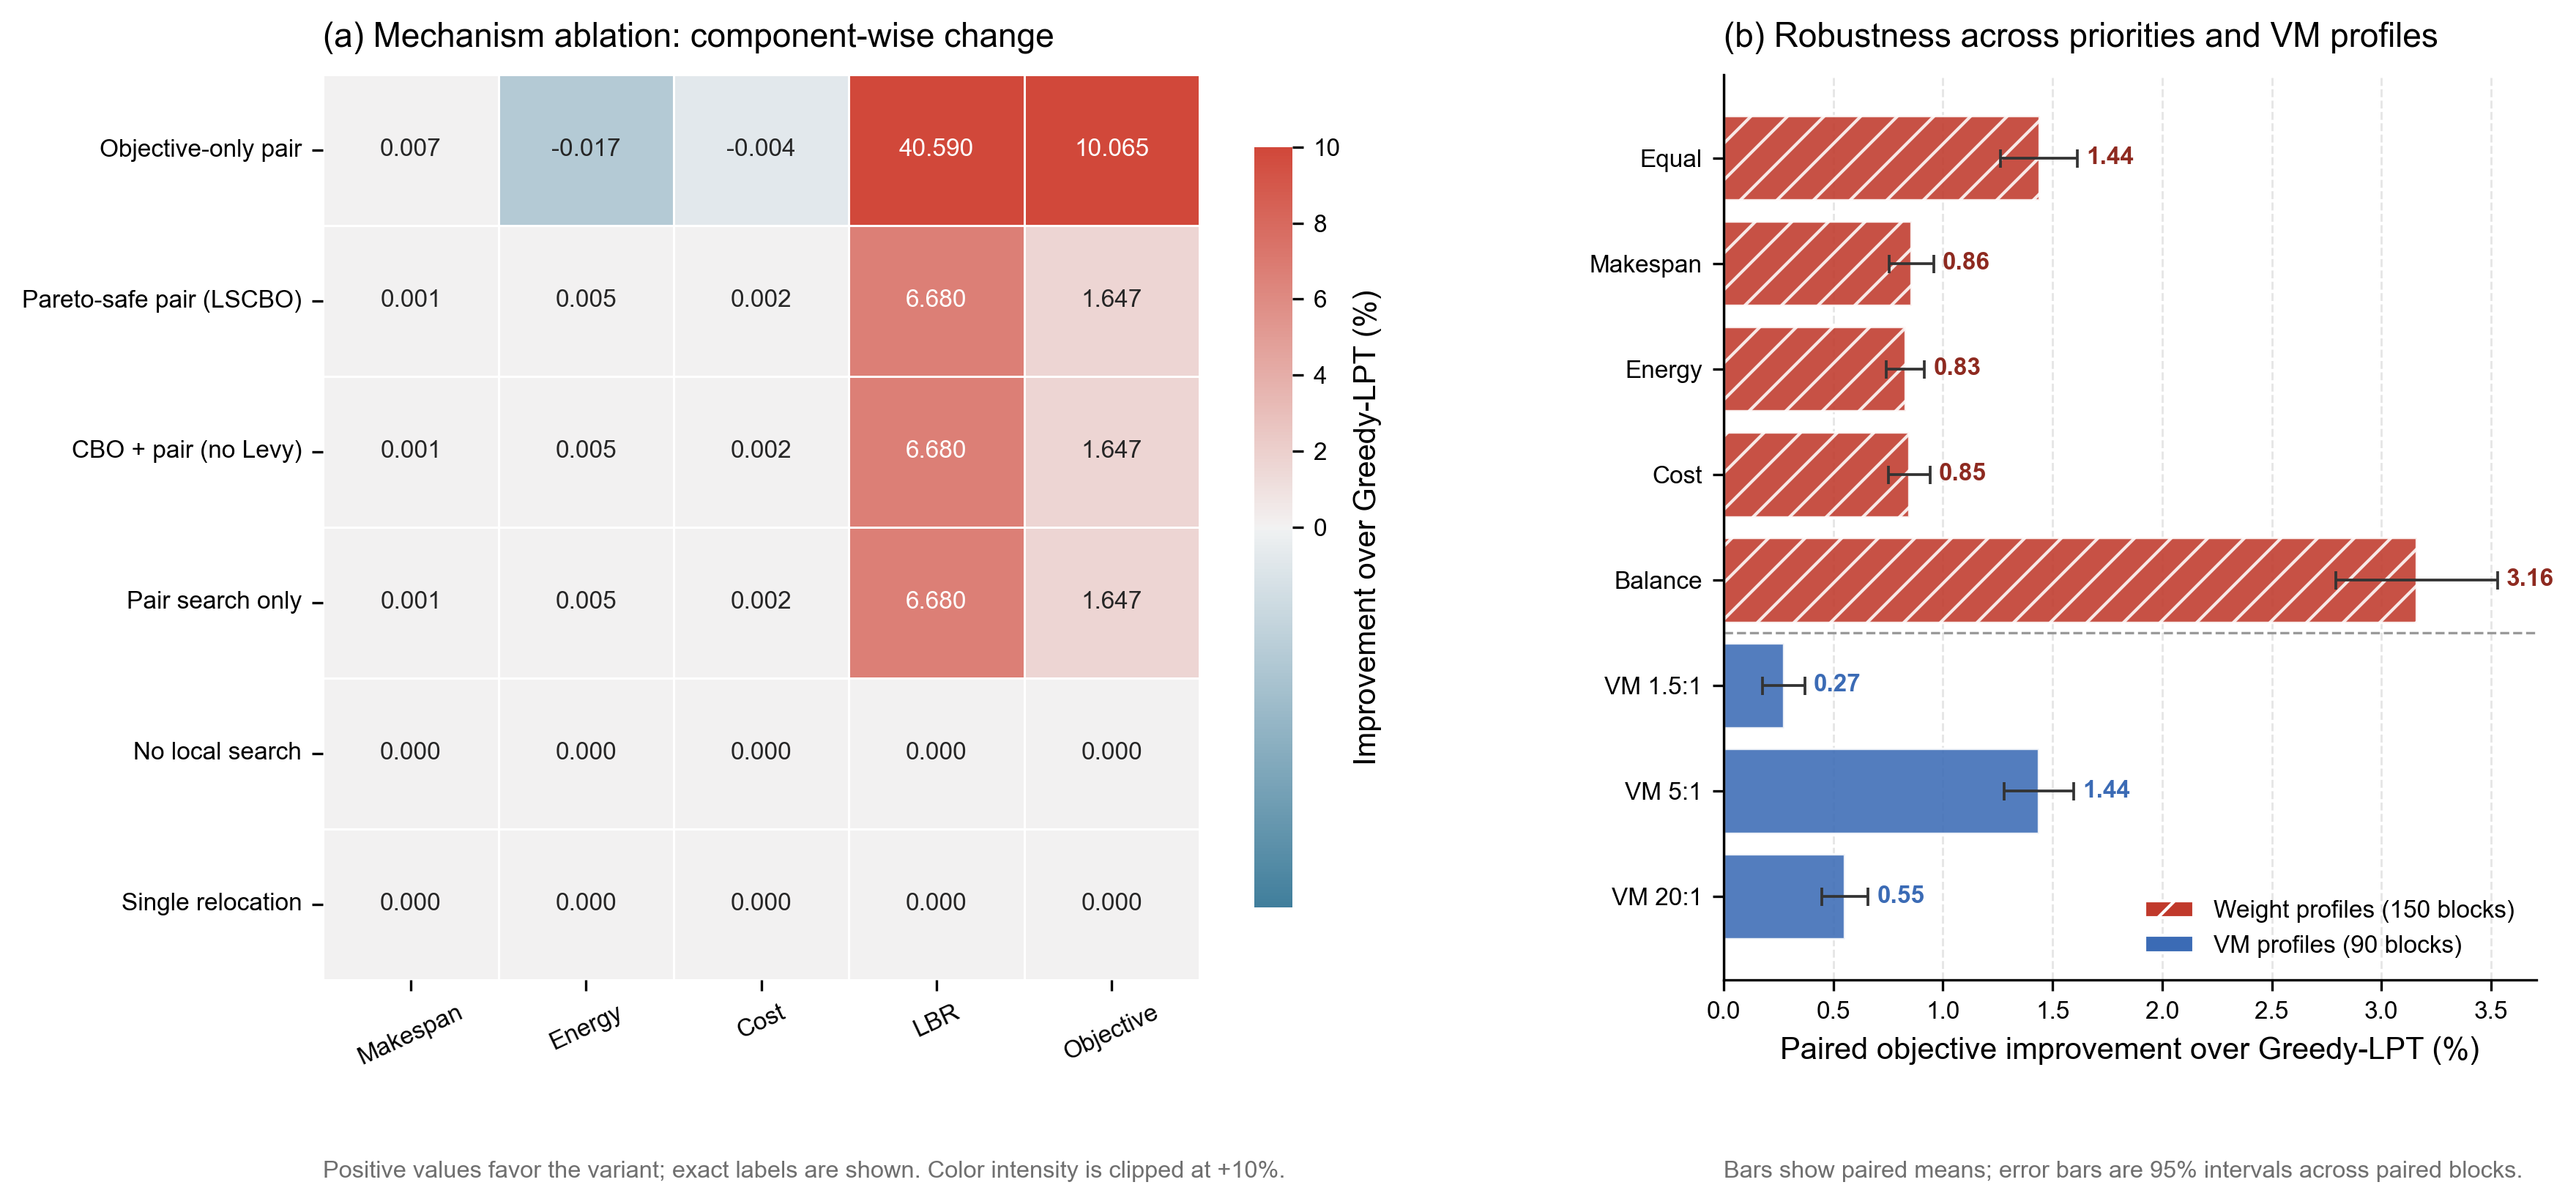
\includegraphics[width=\textwidth]{figures/fig_ablation_robustness.png}
\caption{Mechanism ablation and robustness. (a) Mean component-wise improvement over Greedy-LPT for each ablation variant; positive values favor the variant, exact values are printed, and color intensity is clipped at $+10\%$. (b) Paired mean objective improvement over Greedy-LPT under five weight profiles and three VM-heterogeneity profiles; error bars are 95\% intervals over paired blocks.}\label{fig:ablation_robustness}
\end{figure*}

\section{Discussion}\label{sec6}

The revised experiments change the interpretation of the study. First, Greedy-LPT is a strong baseline: GWO, WOA, and AOA never improve it, while CBO and PSO each improve only one of 150 blocks by a negligible aggregate amount. The cloud evidence therefore provides no support for claiming a repeatable population-search advantage over deterministic scheduling under this protocol. Second, pair reassignment makes a consistent but limited refinement. Its reference-normalized objective benefit ranges from 1.48\% to 1.74\% across scales, while the relative LBR reduction ranges from 5.65\% to 6.81\%. In absolute terms, mean LBR changes from 0.003934 to 0.003671, and physical makespan, energy, and cost reductions remain below 0.01\% overall. Statistical significance is driven by same-signed paired differences and must not be confused with a large operational effect.

The Pareto-safe rule answers an important weakness of scalar acceptance. The objective-only ablation reduces the normalized objective by 10.06\% and LBR by 40.59\%, but worsens energy in 147 blocks and cost in 148 blocks relative to Greedy-LPT. The proposed rule rejects those exchanges and guarantees component-wise non-worsening relative to the incumbent. This guarantee is empirical with respect to the four evaluated components and deterministic by construction for every accepted move.

The host attribution is equally clear in the matched ablation. LSCBO, no-L\'{e}vy CBO with pair search, and pair search alone produce identical cloud results. Thus, the repeatable cloud gain is not explained by L\'{e}vy exploration or by the CBO phases. Their role is limited to the separate continuous benchmark, where the additive L\'{e}vy trial improves CBO on all 29 functions, LSCBO ranks first on average, and LSCBO remains statistically tied with SA under the cross-function analysis.

Several limitations remain. The task model is offline and independent; workflows with precedence constraints, communication costs, failures, and task arrivals are not covered. Workloads are synthetic, use uniformly sampled task lengths, and retain 50 VMs, so the reported seed variation does not represent production traces. The nonlinear power and synthetic monotone price models are controlled analytical approximations rather than measurements from a production datacenter. Scalarization is anchored to the Greedy-LPT value of every criterion; this makes weights comparable within an instance but also makes the reported objective relative to that reference. Greedy-LPT is strong in the tested independent-task setting, which leaves little room for improvement. The pair search uses random sampling rather than exhaustive neighborhood evaluation, and its 5,400 local trials may be unsuitable for latency-critical online decisions. Finally, the study does not compare against exact solvers on small instances or learning-based schedulers. The conclusions are therefore restricted to no-regression refinement of the reported deterministic schedule under the stated model.

\section{Conclusion and Future Work}\label{sec7}

This study presents a Pareto-safe task-pair reassignment mechanism within an LSCBO cloud scheduler. The corrected protocol includes Greedy-LPT as a reported baseline and common warm start, uses a direct decoder, gives every population method the same 6,000-evaluation budget, aligns the LBR formula with the program, and evaluates the continuous benchmark with cross-function statistics.

Across 150 main cloud blocks, pair reassignment lowers the reference-normalized scalar objective in every block without worsening makespan, energy, cost, or LBR. The 1.65\% mean objective reduction is mainly a load-balance refinement; the other physical components change only slightly. Ablation shows that the cloud result belongs to the pair-reassignment operator, not to CBO or L\'{e}vy exploration. On CEC2017, LSCBO has the best average rank among nine methods, but is not significantly different from SA after correction. Future work should test precedence-constrained workflows and real traces, compare against exact small-instance optima, evaluate latency-aware stopping rules, and replace synthetic energy and price functions with calibrated datacenter measurements.

\section*{Statements and Declarations}
\textbf{Funding} No external funding was received for this work.

\textbf{Competing Interests} The authors declare no competing interests.

\textbf{Author Contributions} All authors contributed to the study conception, algorithm design, implementation, experiments, and analysis. The first draft of the manuscript was written by the corresponding author and all authors read and approved the final manuscript.

\textbf{Data Availability} The anonymized reproducibility archive supplied with the submission contains the 5,310-row canonical cloud dataset, the 12-row CloudSim Plus smoke replay, all 7,830 per-run CEC2017 results, aggregate statistical outputs, and verification reports. The public repository for the current submission package is available at \url{https://github.com/Lazywords2006/LSCBO}. Full CloudSim replay of all formal rows is not used for the numerical claims in this version.

\textbf{Code Availability} The anonymized archive and the public repository at \url{https://github.com/Lazywords2006/LSCBO} contain the LSCBO and comparator implementations, CloudSim Plus experiment entry points, result-aggregation scripts, tests, and figure-generation code needed to reproduce the reported analyses.

\textbf{AI Tool Usage} AI-assisted tools were used during manuscript preparation for language editing, consistency checking, and formatting support. All experimental design, data analysis, scientific claims, and final manuscript decisions were reviewed and verified by the authors.

\textbf{Ethics Approval} Not applicable.

\textbf{Consent to Participate} Not applicable.

\textbf{Consent for Publication} Not applicable.

\begin{thebibliography}{45}

\bibitem{Braun2001}
Braun TD, Siegel HJ, Beck N, B\"{o}l\"{o}ni LL, Maheswaran M, Reuther AI, Robertson JP, Theys MD, Yao B, Hensgen D, Freund RF (2001) A comparison of eleven static heuristics for mapping a class of independent tasks onto heterogeneous distributed computing systems. J Parallel Distrib Comput 61(6):810--837. \url{https://doi.org/10.1006/jpdc.2000.1714}

\bibitem{Etminani2007}
Etminani K, Naghibzadeh M (2007) A Min-Min Max-Min selective algorithm for grid task scheduling. Proc 3rd IEEE/IFIP Int Conf Cent Asia Internet 1--7. \url{https://doi.org/10.1109/CANET.2007.4401694}

\bibitem{Mirjalili2016}
Mirjalili S, Lewis A (2016) The whale optimization algorithm. Adv Eng Softw 95:51--67. \url{https://doi.org/10.1016/j.advengsoft.2016.01.008}

\bibitem{Mirjalili2014}
Mirjalili S, Mirjalili SM, Lewis A (2014) Grey wolf optimizer. Adv Eng Softw 69:46--61. \url{https://doi.org/10.1016/j.advengsoft.2013.12.007}

\bibitem{Xue2022}
Xue J, Shen B (2023) Dung beetle optimizer: a new meta-heuristic algorithm for global optimization. J Supercomput 79:7305--7336. \url{https://doi.org/10.1007/s11227-022-04959-6}

\bibitem{Abualigah2021}
Abualigah L, Diabat A, Mirjalili S, Elaziz MA, Gandomi AH (2021) The arithmetic optimization algorithm. Comput Methods Appl Mech Eng 376:113609. \url{https://doi.org/10.1016/j.cma.2020.113609}

\bibitem{Khatab2025}
Khatab M, El-Gamel M, Saleh AI, El-Shenawy A, Rabie AH (2025) Coyote and Badger Optimization (CBO): a natural inspired meta-heuristic algorithm based on cooperative hunting. Commun Nonlinear Sci Numer Simul 140:108333. \url{https://doi.org/10.1016/j.cnsns.2024.108333}

\bibitem{Chintale2024}
Chintale P, Malviya RK, Merla NB, Chinna PPG, Desaboyina G, Sure TAR (2024) Levy flight osprey optimization algorithm for task scheduling in cloud computing. Proc 2024 Int Conf Intell Algorithms Comput Intell Syst (IACIS) 1--5. \url{https://doi.org/10.1109/IACIS61494.2024.10721633}

\bibitem{Sabipour2025}
Sabipour MR, Sayadnavard MH (2025) A chaotic RIME optimization algorithm based on generalized quadratic interpolation with L\'{e}vy flight for task scheduling in cloud computing. J Soft Comput Inf Technol 14(1):57--67. \url{https://doi.org/10.22034/jscit.2025.220413}

\bibitem{Zhu2025}
Zhu M, Li J, Yang X (2025) A hybrid SAO and RIME optimizer for global optimization and cloud task scheduling. Biomimetics 10(10):690. \url{https://doi.org/10.3390/biomimetics10100690}

\bibitem{Xie2024}
Xie R, Li S, Wu F, Wu L, Xiong X (2024) An enhanced dung beetle optimizer for cloud task schedule. Proc 4th Int Conf Appl Math Model Intell Comput (CAMMIC 2024) 13219:80. \url{https://doi.org/10.1117/12.3036506}

\bibitem{Wolpert1997}
Wolpert DH, Macready WG (1997) No free lunch theorems for optimization. IEEE Trans Evol Comput 1(1):67--82. \url{https://doi.org/10.1109/4235.585893}

\bibitem{Kennedy1995}
Kennedy J, Eberhart R (1995) Particle swarm optimization. Proc ICNN'95-Int Conf Neural Networks 4:1942--1948. \url{https://doi.org/10.1109/ICNN.1995.488968}

\bibitem{Goldberg1989}
Goldberg D.E. (1989) Genetic algorithms in search, optimization, and machine learning. Addison-Wesley.

\bibitem{Kirkpatrick1983}
Kirkpatrick S, Gelatt Jr CD, Vecchi MP (1983) Optimization by simulated annealing. Science 220(4598):671--680. \url{https://doi.org/10.1126/science.220.4598.671}

\bibitem{Deb2002}
Deb K, Pratap A, Agarwal S, Meyarivan T (2002) A fast and elitist multiobjective genetic algorithm: NSGA-II. IEEE Trans Evol Comput 6(2):182--197. \url{https://doi.org/10.1109/4235.996017}

\bibitem{Zhang2007}
Zhang Q, Li H (2007) MOEA/D: a multiobjective evolutionary algorithm based on decomposition. IEEE Trans Evol Comput 11(6):712--731. \url{https://doi.org/10.1109/TEVC.2007.892759}

\bibitem{Tasgetiren2007}
Tasgetiren MF, Liang YC, \c{S}evkli M, Gencyilmaz G (2007) A particle swarm optimization algorithm for makespan and total flowtime minimization in the permutation flowshop sequencing problem. Eur J Oper Res 177(3):1930--1947. \url{https://doi.org/10.1016/j.ejor.2005.12.024}

\bibitem{AbdelBasset2023}
Abdel-Basset M, Mohamed R, Azeem SAA, Jameel M, Abouhawwash M (2023) Kepler optimization algorithm: a new metaheuristic algorithm inspired by Kepler's laws of planetary motion. Knowl-Based Syst 268:110454. \url{https://doi.org/10.1016/j.knosys.2023.110454}

\bibitem{Qian2025}
Qian Z, Zhang Y, Pu DQ, Xie G, Pu D, Ye M (2025) A new hybrid improved Kepler optimization algorithm based on multi-strategy fusion and its applications. Mathematics 13(3):405. \url{https://doi.org/10.3390/math13030405}

\bibitem{Hashim2022}
Hashim FA, Hussien AG (2022) Snake optimizer: a novel meta-heuristic optimization algorithm. Knowl-Based Syst 242:108320. \url{https://doi.org/10.1016/j.knosys.2022.108320}

\bibitem{Deng2023}
Deng L, Liu S (2023) Snow ablation optimizer: a novel metaheuristic technique for numerical optimization and engineering design. Expert Syst Appl 225:120069. \url{https://doi.org/10.1016/j.eswa.2023.120069}

\bibitem{Trojovska2022}
Trojovsk\'{y} P, Dehghani M (2022) Pelican optimization algorithm: a novel nature-inspired algorithm for engineering applications. Sensors 22(3):855. \url{https://doi.org/10.3390/s22030855}

\bibitem{Faramarzi2020}
Faramarzi A, Heidarinejad M, Mirjalili S, Gandomi AH (2020) Marine Predators Algorithm: a nature-inspired metaheuristic. Expert Syst Appl 152:113377. \url{https://doi.org/10.1016/j.eswa.2020.113377}

\bibitem{Abualigah2022}
Abualigah L, Elaziz MA, Sumari P, Geem ZW, Gandomi AH (2022) Reptile Search Algorithm (RSA): a nature-inspired meta-heuristic optimizer. Expert Syst Appl 191:116158. \url{https://doi.org/10.1016/j.eswa.2021.116158}

\bibitem{Wang2022}
Wang L, Cao Q, Zhang Z, Mirjalili S, Zhao W (2022) Artificial rabbits optimization: a new bio-inspired meta-heuristic algorithm for solving engineering optimization problems. Eng Appl Artif Intell 114:105082. \url{https://doi.org/10.1016/j.engappai.2022.105082}

\bibitem{Ghafari2023}
Ghafari R, Mansouri N (2023) E-AVOA-TS: enhanced African vultures optimization algorithm-based task scheduling strategy for fog--cloud computing. Sustain Comput Inform Syst 40:100918. \url{https://doi.org/10.1016/j.suscom.2023.100918}

\bibitem{Ferahtia2023}
Ferahtia S, Houari A, Rezk H, Djerioui A, Machmoum M, Motahhir S, Ait-Ahmed M (2023) Red-tailed hawk algorithm for numerical optimization and real-world problems. Sci Rep 13:12950. \url{https://doi.org/10.1038/s41598-023-38778-3}

\bibitem{Qin2024}
Qin X, Li S, Tong J, Xie C, Zhang X, Wu F, Xie Q, Ling Y, Lin G (2024) ERTH scheduler: enhanced red-tailed hawk algorithm for multi-cost optimization in cloud task scheduling. Artif Intell Rev 57:328. \url{https://doi.org/10.1007/s10462-024-10945-6}

\bibitem{EbrahimiMood2025}
Ebrahimi Mood S, Souri A, Inanc N, Li KC (2025) CEEO: an innovative Coulomb-enhanced equilibrium optimizer for task scheduling of cloud services in IoT environments. Computing 107:138. \url{https://doi.org/10.1007/s00607-025-01495-y}

\bibitem{Dehghani2023}
Dehghani M, Trojovsk\'{y} P (2023) Osprey optimization algorithm: a new bio-inspired metaheuristic algorithm for solving engineering optimization problems. Front Mech Eng 8:1126450. \url{https://doi.org/10.3389/fmech.2022.1126450}

\bibitem{Mantegna1994}
Mantegna RN (1994) Fast, accurate algorithm for numerical simulation of L\'{e}vy stable stochastic processes. Phys Rev E 49(5):4677--4683. \url{https://doi.org/10.1103/PhysRevE.49.4677}

\bibitem{Yang2009}
Yang XS, Deb S (2009) Cuckoo search via L\'{e}vy flights. Proc 2009 World Congr Nat Biol Inspired Comput (NaBIC) 210--214. \url{https://doi.org/10.1109/NABIC.2009.5393690}

\bibitem{Moscato1989}
Moscato P (1989) On evolution, search, optimization, genetic algorithms and martial arts: towards memetic algorithms. Caltech Concurrent Computation Program, C3P Report 826.

\bibitem{Kiliaan1991}
Kiliaan H, Mamo C, Paquet P (1991) A coyote, Canis latrans, and badger, Taxidea taxus, interaction near Cypress Hills Provincial Park, Alberta. Can Field-Nat 105(1):122--123. \url{https://doi.org/10.5962/p.357965}

\bibitem{Mao2016}
Mao H, Alizadeh M, Menache I, Kandula S (2016) Resource management with deep reinforcement learning. Proc 15th ACM Workshop Hot Topics Netw (HotNets) 50--56. \url{https://doi.org/10.1145/3005745.3005750}

\bibitem{Mao2019}
Mao H, Schwarzkopf M, Bojja Venkatakrishnan S, Meng Z, Alizadeh M (2019) Learning scheduling algorithms for data processing clusters. Proc ACM SIGCOMM 2019 270--288. \url{https://doi.org/10.1145/3341302.3342080}

\bibitem{CEC2017}
Awad NH, Ali MZ, Liang JJ, Qu BY, Suganthan PN (2016) Problem definitions and evaluation criteria for the CEC 2017 special session and competition on single objective bound constrained real-parameter numerical optimization. Nanyang Technological University, Tech. Rep.

\bibitem{Dehghani2022HLBO}
Dehghani M, Trojovsk\'{y} P (2022) Hybrid leader based optimization: a new stochastic optimization algorithm for solving optimization applications. Sci Rep 12:5549. \url{https://doi.org/10.1038/s41598-022-09514-0}

\bibitem{Guan2023GWCA}
Guan Z, Ren C, Niu J, Wang P, Shang Y (2023) Great Wall Construction Algorithm: a novel meta-heuristic algorithm for engineer problems. Expert Syst Appl 233:120905. \url{https://doi.org/10.1016/j.eswa.2023.120905}

\bibitem{Friedman1937}
Friedman M (1937) The use of ranks to avoid the assumption of normality implicit in the analysis of variance. J Am Stat Assoc 32(200):675--701. \url{https://doi.org/10.1080/01621459.1937.10503522}

\bibitem{ImanDavenport1980}
Iman RL, Davenport JM (1980) Approximations of the critical region of the Friedman statistic. Commun Stat--Theory Methods 9(6):571--595. \url{https://doi.org/10.1080/03610928008827904}

\bibitem{Wilcoxon1945}
Wilcoxon F (1945) Individual comparisons by ranking methods. Biometrics Bull 1(6):80--83. \url{https://doi.org/10.2307/3001968}

\bibitem{Calheiros2011}
Calheiros RN, Ranjan R, Beloglazov A, De Rose CAF, Buyya R (2011) CloudSim: a toolkit for modeling and simulation of cloud computing environments and evaluation of resource provisioning algorithms. Softw Pract Exp 41(1):23--50. \url{https://doi.org/10.1002/spe.995}

\bibitem{SilvaFilho2017}
Silva Filho MC, Oliveira RL, Monteiro CC, Inacio PRM, Freire MM (2017) CloudSim Plus: a cloud computing simulation framework pursuing software engineering principles for improved modularity, extensibility and correctness. Proc 2017 IFIP/IEEE Symp Integr Netw Serv Manag (IM) 400--406. \url{https://doi.org/10.23919/INM.2017.7987304}
\end{thebibliography}

\end{document}
